% This example is meant to be compiled with lualatex or xelatex
% The theme itself also supports pdflatex
\PassOptionsToPackage{unicode}{hyperref}
\documentclass[aspectratio=1610, 9pt]{beamer}

% Load packages you need here
\usepackage[english]{babel}

\usepackage{csquotes}

\usepackage{tikz}\usetikzlibrary{arrows.meta,calc,positioning}

\usepackage{amsmath}
\usepackage{amssymb}
\usepackage{mathtools}

\usepackage{hyperref}
\usepackage{bookmark}

% load the theme after all packages

\usetheme[
  % showtotalframes, % show total number of frames in the footline
  % dark, % optional dark theme, uncomment to use
]{tudo}


% Put settings here, like
\unimathsetup{
  math-style=ISO,
  bold-style=ISO,
  nabla=upright,
  partial=upright,
  mathrm=sym,
}

%\title{Direction Reconstruction for CTAO}
\title{Stereoscopic direction reconstruction algorithms for CTAO}
\author[A.~Aki]{Akram Aki}
\date{November, 20, 2025}
\institute[Elsässer/Rhode]{Working Group Elsässer/Rhode}
\titlegraphic{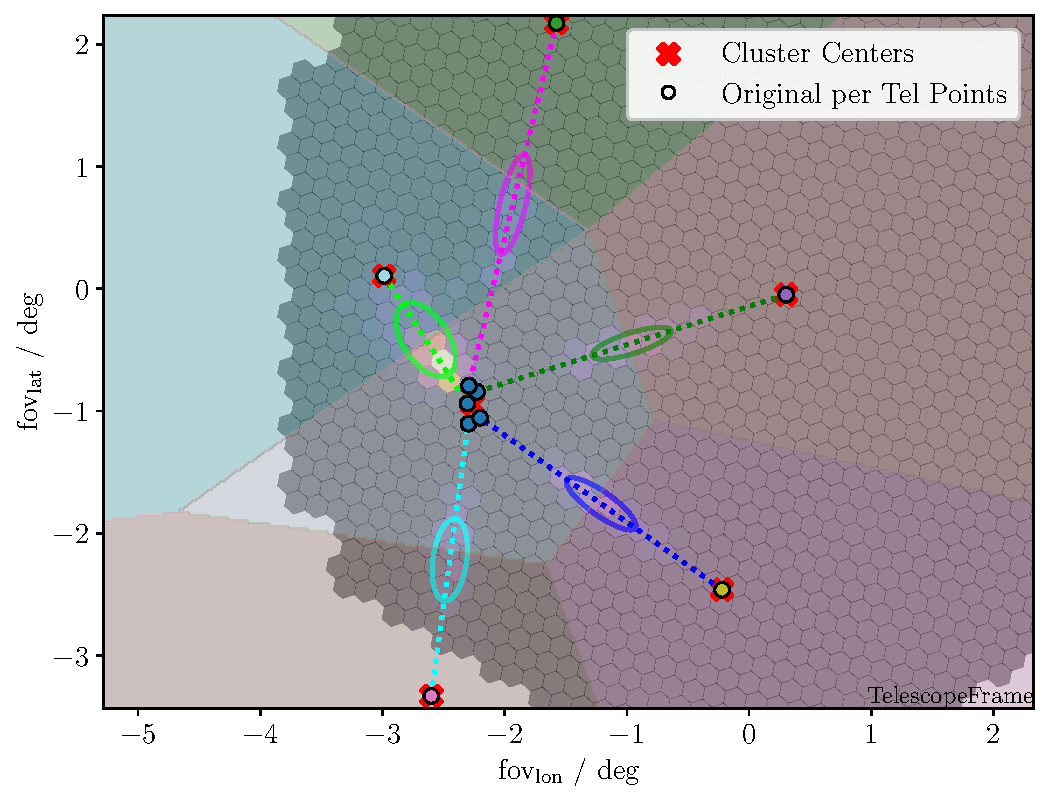
\includegraphics[clip, trim=2cm 3cm 2cm 3cm, width=0.55\textwidth]{images/KMeans_fullView.pdf}}

\begin{document}

\maketitle

\begin{frame}{Overview}
  \tableofcontents
\end{frame}

\section{Thesis Overview}
\begin{frame}{Thesis Overview}
  \begin{itemize}
    \setlength{\itemsep}{0.7cm} % increase space between items
    \item This thesis was conducted within the field of \textbf{gamma-ray astronomy}.  
    \item The goal is to improve how we \textbf{reconstruct the arrival direction of cosmic gamma rays} detected by ground-based telescopes.  
    \item The work focuses on the \textbf{Cherenkov Telescope Array Observatory (CTAO)}, the next-generation gamma-ray observatory.  
    \item Two new methods were developed to \textbf{enhance reconstruction accuracy}.  
  \end{itemize}
\end{frame}

% --- SPEAKER NOTES ---
%“Good morning, and thank you for being here.
%Today, I’m presenting the results of my bachelor’s thesis.
%
%My work is situated in gamma-ray astronomy, which studies extremely energetic processes in the universe.
%Specifically, I worked on improving how we reconstruct the direction from which a detected gamma ray came 
%To achieve this, I developed and compared two new reconstruction methods.
%Before going into the technical details, I’ll start by motivating why gamma rays are interesting in the first place.”

%%%%%%%%%%%%%%%%

% =======================
% MOTIVATION SECTION
% =======================

\section{Motivation}

\begin{frame}{Motivation: Why High-Energy Gamma Rays?}
  \begin{columns}[c, totalwidth=\textwidth]
    % Left column: text (slightly narrower)
    \begin{column}{0.35\textwidth}
      \begin{itemize}
        \item Gamma rays are the \textbf{most energetic form of light}.  
        \item Produced in \textbf{extreme cosmic environments}:  
          \begin{itemize}
            \item Supernova explosions  
            \item Pulsar wind nebulae  
            \item Black holes
            \item Active galaxies 
          \end{itemize}
        \item They reveal processes that cannot be studied in laboratories on Earth. 
        \item The non thermal universe is oberservable using gamma rays 
      \end{itemize}
    \end{column}

    % Right column: larger image
    \begin{column}{0.65\textwidth}
      \centering
      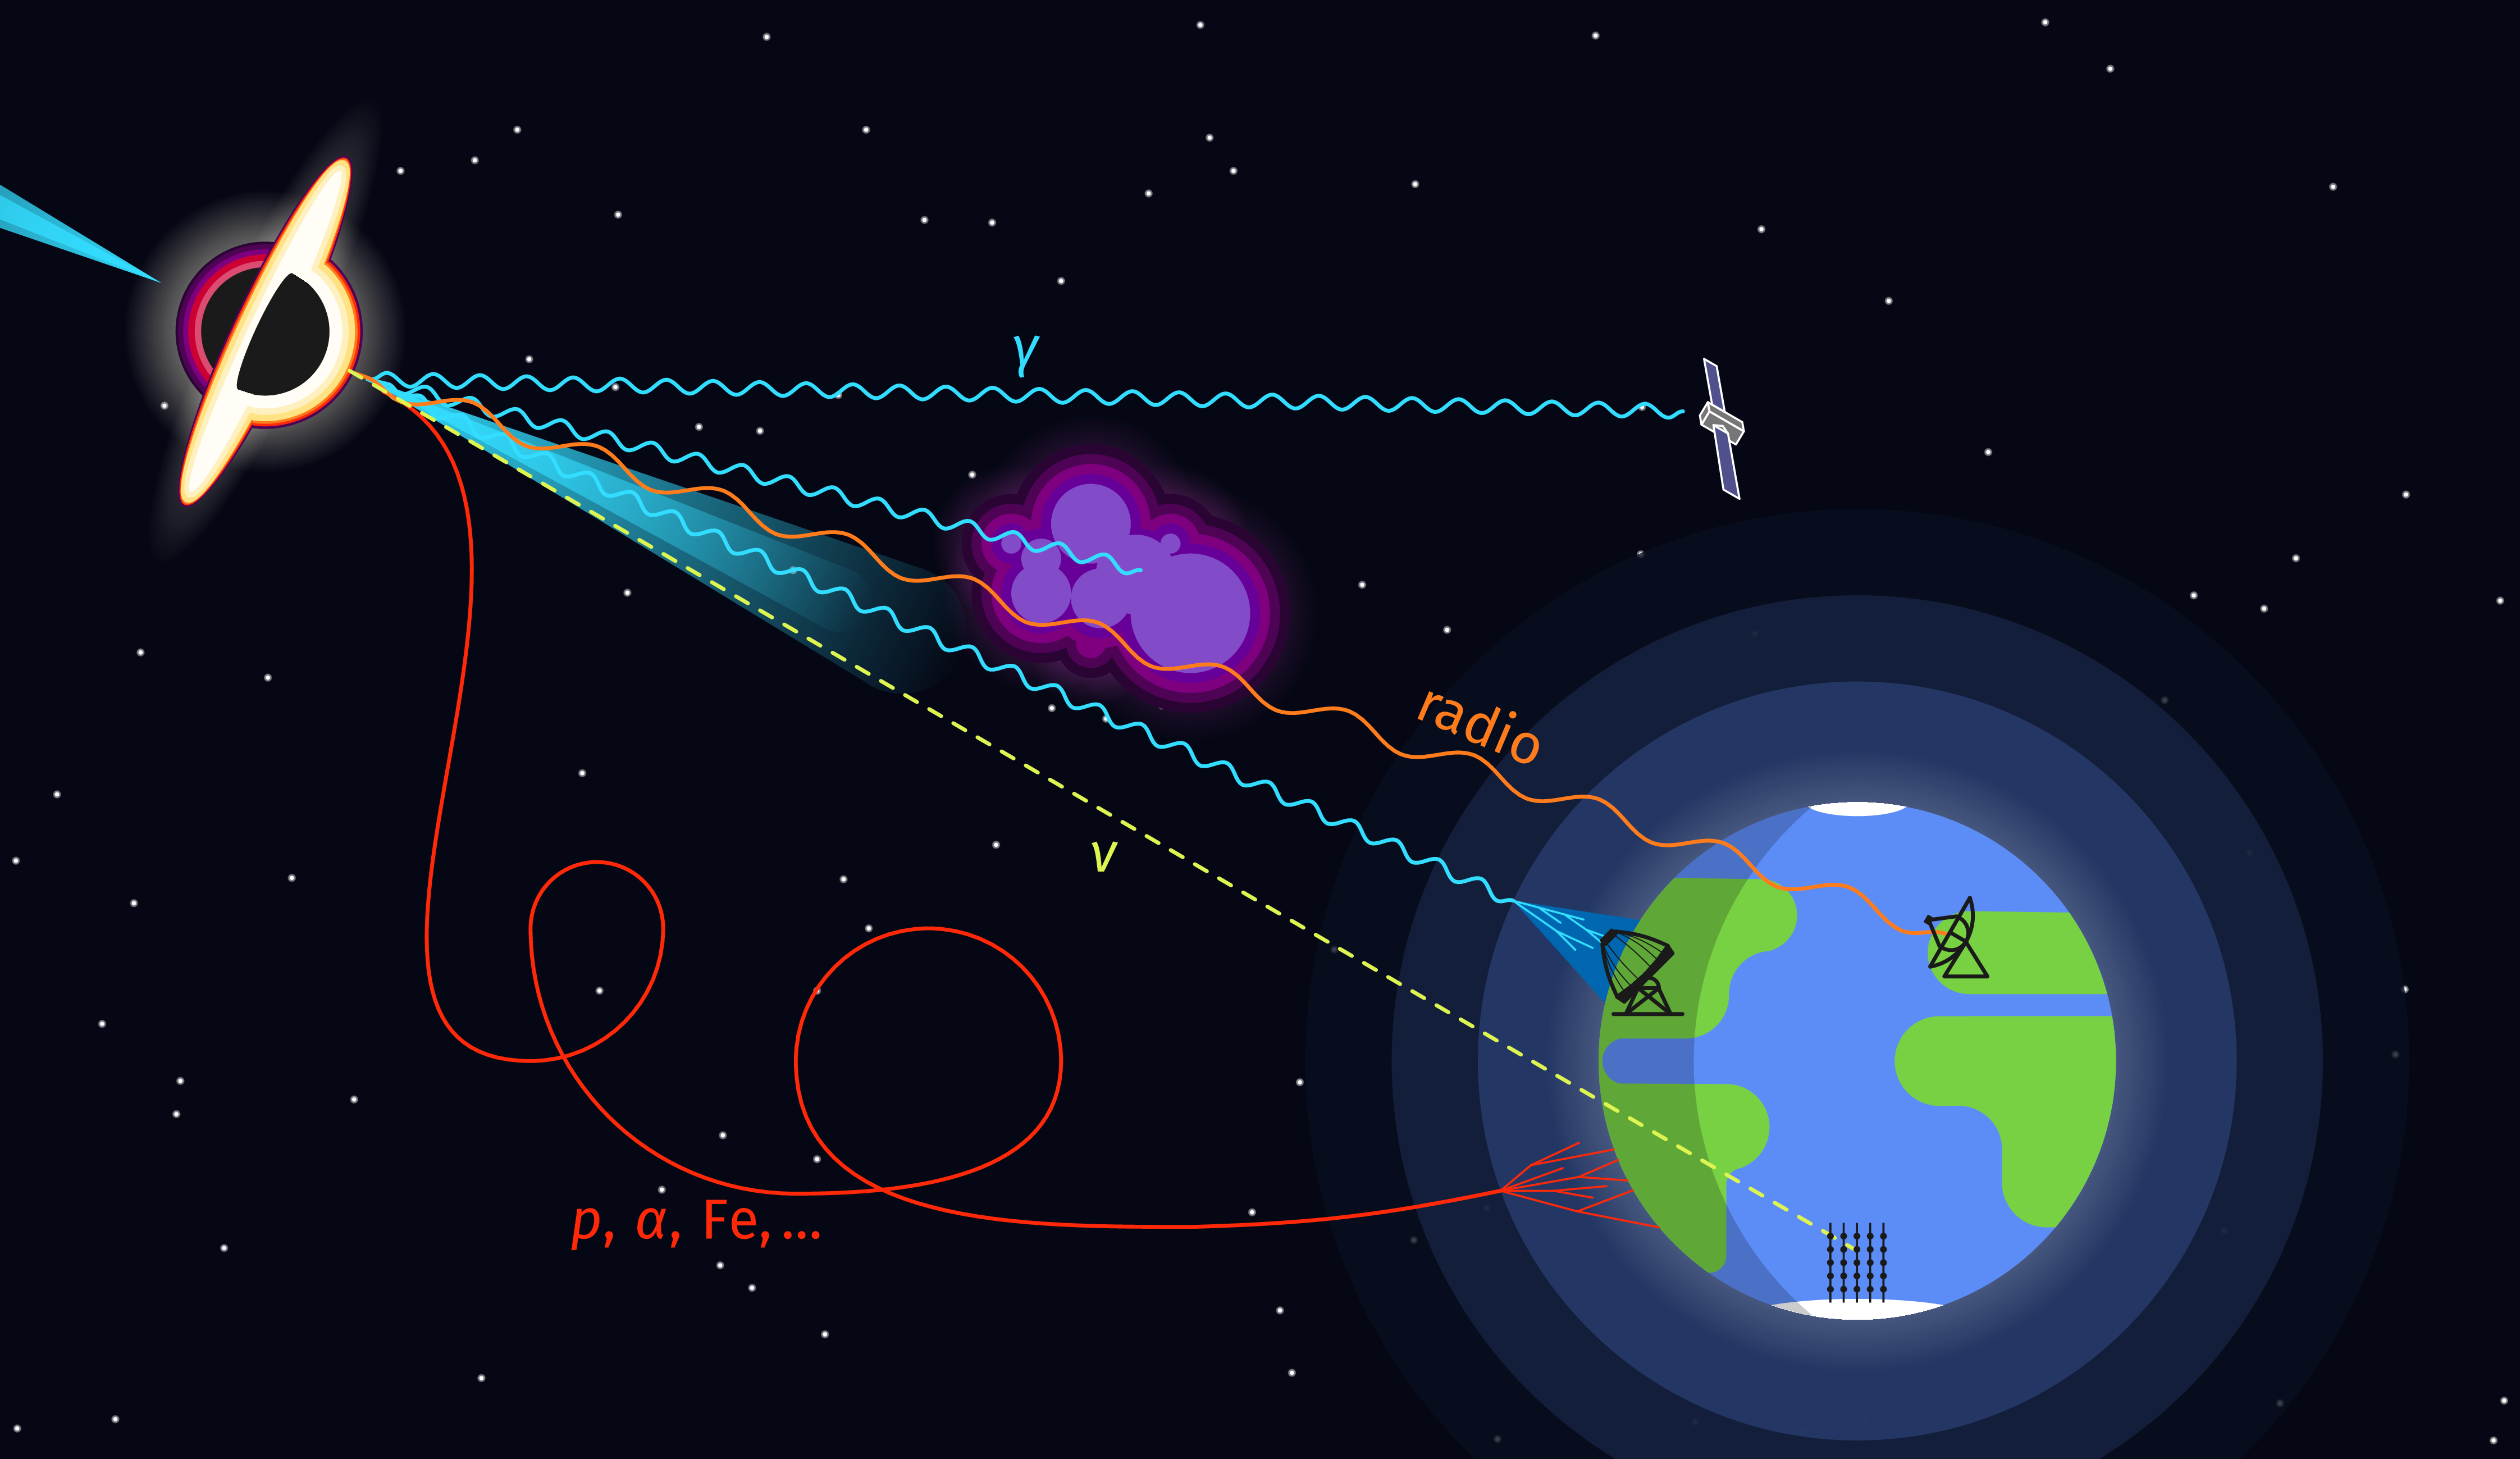
\includegraphics[width=\textwidth]{images/gammaRayOrigin.png}
      \vspace{2mm}
      {\footnotesize Origins of high-energy gamma rays in the universe [adapted from A. Knierim].}
    \end{column}
  \end{columns}
\end{frame}

% --- SPEAKER NOTES ---
% "In astrophysics, we study the most extreme places in the universe—
% black holes, neutron stars, supernovae. These regions accelerate particles
% to energies far higher than we can reach with any experiment on Earth.
% Gamma rays are the light produced in these processes, so detecting them
% lets us look directly into those environments."

% -------------------------------------------------------

\section{Imaging Atmospheric Cherenkov Telescopes}

\begin{frame}{Meassuring gamma rays on Earth}
  \begin{center}
    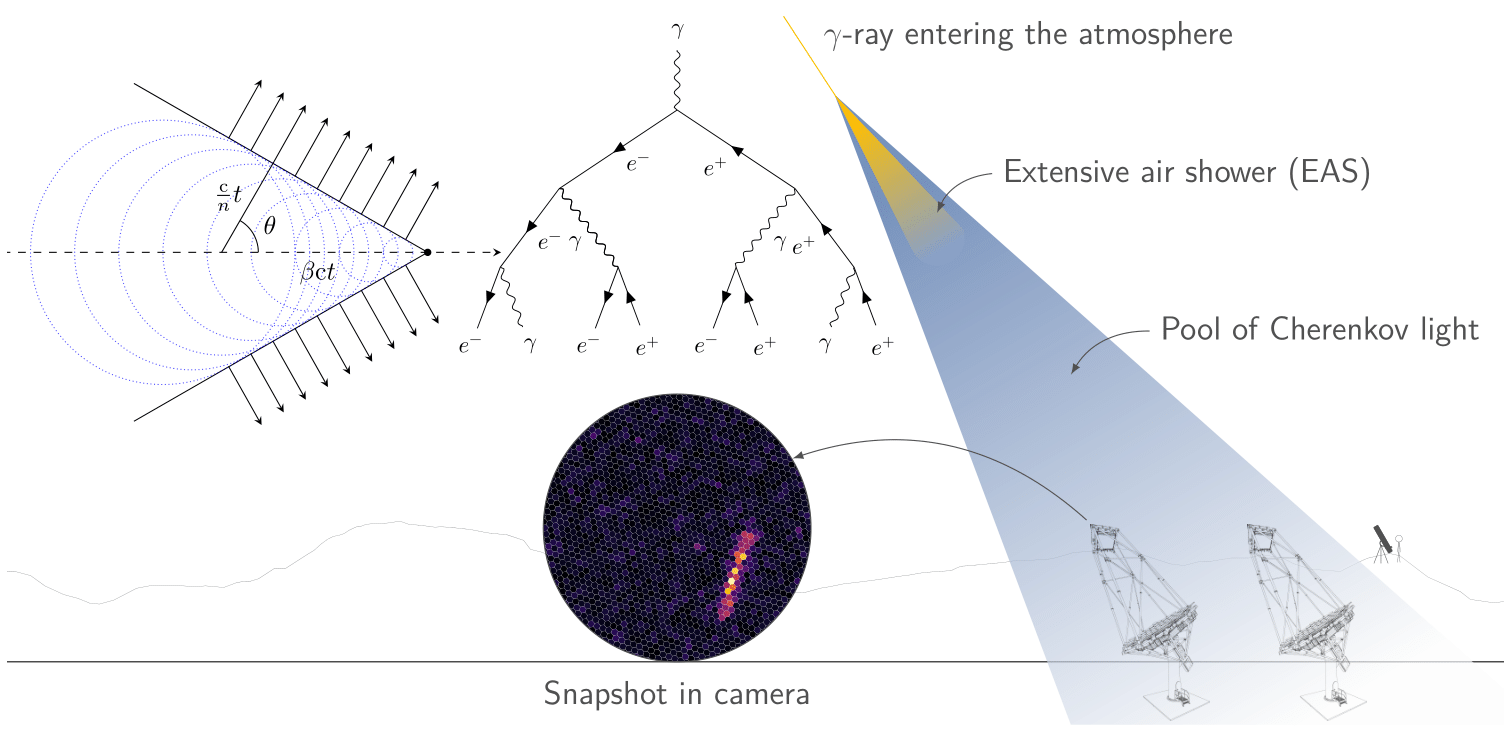
\includegraphics[width=0.85\textwidth]{images/IACT.png}
    \newline
    {\footnotesize [adapted from A. Knierim]}
  \end{center}
\end{frame}
% --- SPEAKER NOTES ---
% "Gamma rays are absorbed by the atmosphere—good for life, bad for astronomy.
% But when they interact with air molecules, they create a cascade of secondary
% particles moving faster than light in air. This produces a very faint, blue flash
% of Cherenkov light, which lasts only a few nanoseconds. We detect these flashes
% with large mirrors on the ground—Cherenkov telescopes."

% -------------------------------------------------------

\begin{frame}{\textbf{Cherenkov Telescope Array Observatory (CTAO)}}
  \begin{itemize}
    \item CTAO will be the next-generation ground-based gamma-ray facility.  
    \item It aims to, among other goals, produce the most precise \textbf{gamma-ray sky maps} ever.  
    \item Better direction reconstruction = sharper sources, higher sensitivity, and more discoveries.  
  \end{itemize}
  \begin{center}
    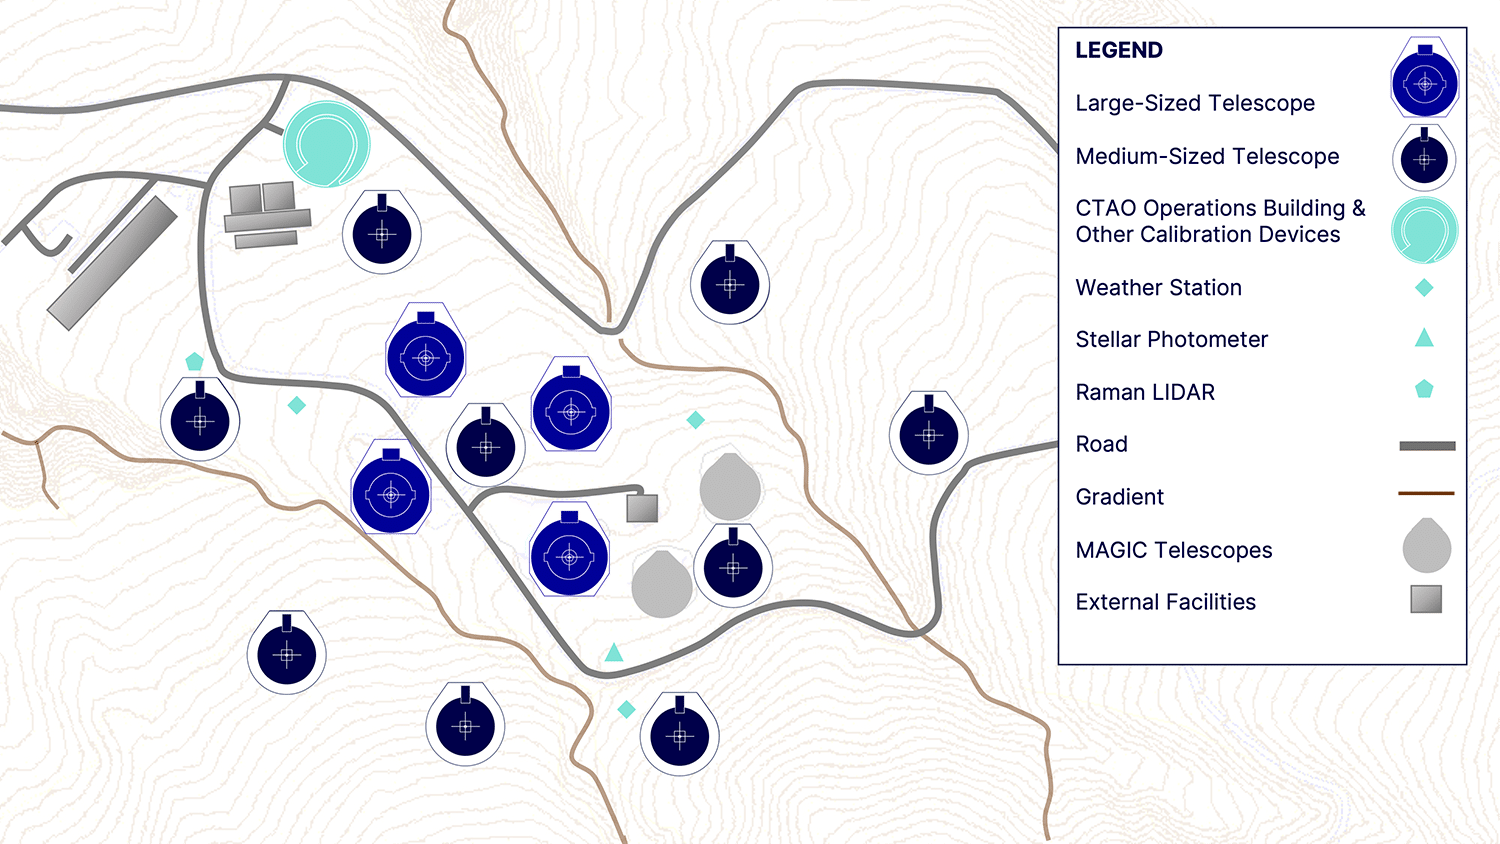
\includegraphics[width=0.65\textwidth]{images/CTAO_North_layout.png}
    \newline
    {\footnotesize Layout of the CTAO North site (La Palma) [Adapted from the CTAO Website]}
  \end{center}
\end{frame}
% --- SPEAKER NOTES ---
% "All of this work supports the upcoming CTAO—an international project that
% will use over 100 telescopes on two sites to map the gamma-ray sky.
% The accuracy of direction reconstruction determines how sharp our sky maps are,
% so by improving it, we increase the scientific potential of the observatory."

%\begin{frame}{How We Detect Gamma Rays}
%  \begin{itemize}
%    \item The \textbf{Imaging Atmospheric Cherenkov Technique (IACT)} detects Cherenkov flashes.  
%    \item Each telescope has:  
%      \begin{itemize}
%        \item A large mirror (to collect faint light).  
%        \item A fast camera (to record nanosecond flashes).  
%      \end{itemize}
%    \item Multiple telescopes observe the same air shower from different angles.
%    \item Each telescope can be used to create monoscopic predictions.
%    \item Combining multiple telescope views = \textbf{stereoscopic reconstruction}.  
%  \end{itemize}
%\end{frame}

\begin{frame}{Dataprocessing in CTA Pipe}
  \begin{center}
    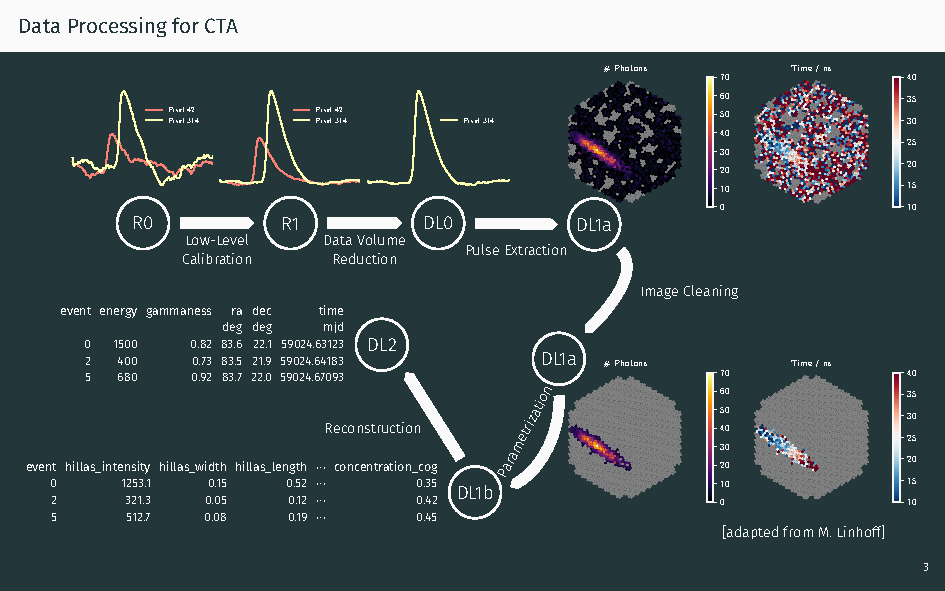
\includegraphics[clip, trim=0cm 0.8cm 0cm 1cm, width=0.9\textwidth]{images/DataProcessing.pdf}
  \end{center}
\end{frame}

% --- SPEAKER NOTES ---
% "Cherenkov telescopes work like ultra-fast cameras that capture the faint blue light
% from air showers. Each telescope collects light with a large mirror and focuses it
% onto a sensitive camera. Since the flash lasts only a few nanoseconds, we need
% very fast electronics. Using several telescopes gives us multiple viewpoints,
% which we later combine to reconstruct the direction of the incoming gamma ray."

\begin{frame}{Example: What a Telescope Sees}
  \begin{columns}[c, totalwidth=\textwidth]
    % Left column: text
    \begin{column}{0.55\textwidth}
      \begin{itemize}
        \setlength{\itemsep}{0.6cm} % increase space between items
        \item The recorded image is a \textbf{streak or ellipse} of light.  
        \item Its shape depends on:  
          \begin{itemize}
            \setlength{\itemsep}{0.4cm} % increase space between items
            \item The geometry of the air shower.  
            \item The distance of the telescope from the shower axis.  
            \item The energy of the gamma-ray.
          \end{itemize}
        \item From this shape, we can estimate the \textbf{source direction}.  
      \end{itemize}
    \end{column}

    % Right column: image
    \begin{column}{0.45\textwidth}
      \centering
      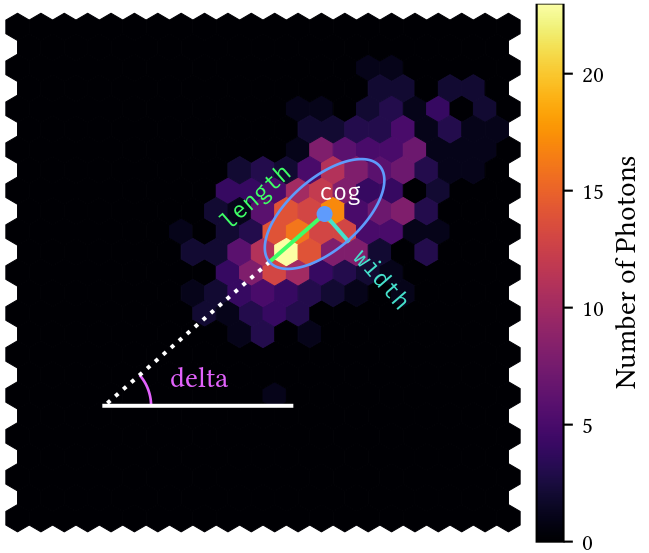
\includegraphics[width=\textwidth]{images/hillas_image.png}
      \vspace{2mm}
      {\footnotesize Example shower image with Hillas parameters [adapted from M. Linhoff].}
    \end{column}
  \end{columns}
\end{frame}

% --- SPEAKER NOTES ---
% "Each telescope records a faint, elongated ellipse.
% The orientation of this ellipse points roughly back to where the gamma ray came from.
% This is described by the so-called Hillas parameters—length, width, and orientation.
% Using these parameters, we can reconstruct the incoming direction."

% -------------------------------------------------------

\begin{frame}{The DISP Method}
  \begin{columns}[c, totalwidth=\textwidth]
    % Left column: text
    \begin{column}{0.55\textwidth}
      \begin{itemize}
        \setlength{\itemsep}{0.3cm} % increase space between items
        \item \textbf{DISP} = distance from the image center to the true source along the main axis.  
        \item Each telescope provides such an estimate using a random forest based on image features.  
        \item Ambiguity: the source can lie at the \textbf{head or tail} of the ellipse.  
        \item A \textbf{Machine Learning classifier} helps choose the correct side (for the monoscopic case).  
        \item For stereoscopic reconstruction the sign ambiguity is solved by the combiner.
      \end{itemize}
    \end{column}

    % Right column: image
    \begin{column}{0.45\textwidth}
      \centering
      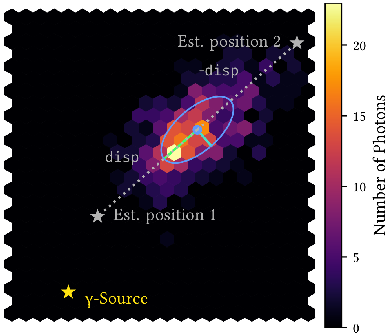
\includegraphics[width=\textwidth]{images/dispMethod.pdf}
      \vspace{2mm}
      {\footnotesize Disp Distance Example Visualization [adapted from M. Linhoff].}
    \end{column}
  \end{columns}
\end{frame}

\begin{frame}{The Reconstruction Challenge}
  \begin{columns}[c, totalwidth=\textwidth]
    % Left column: text
    \begin{column}{0.55\textwidth}
      \begin{itemize}
        \setlength{\itemsep}{0.24cm} % increase space between items
        \item Each telescope recods an image from which we can estimate the gamma-ray’s \textbf{arrival direction}.  
        \item Combining multiple telescope views effectily .  
        \item My thesis: \textbf{improving this direction reconstruction for CTAO}.  
      \end{itemize}
      \vspace{4mm}
      Picture Description:\\
      Yellow star is reconstruction target. \\
      Green crosses are per telescope selected points used for reconstruction/prediction.  \\
      Red crosses are per telescope rejected points not to be used for reconstruction/prediction.  \\
      Green dot is the prediction.
    \end{column}

    % Right column: image
    \begin{column}{0.45\textwidth}
      \centering
      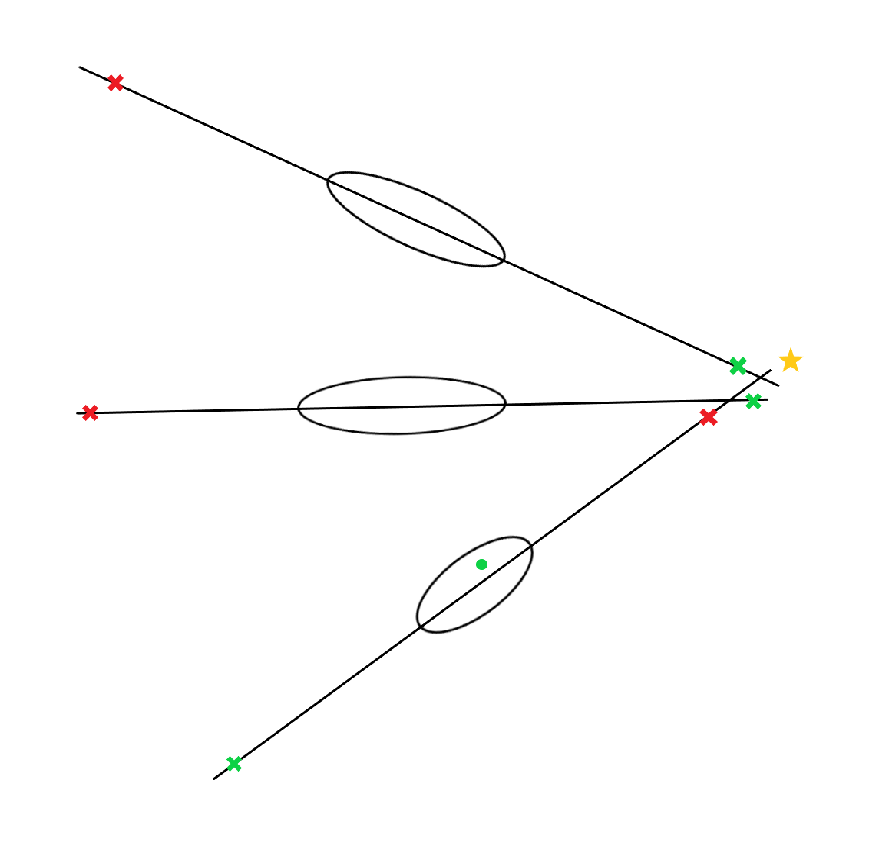
\includegraphics[width=\textwidth]{images/reconstruction_problem.pdf}
      \vspace{2mm}
      {\footnotesize [adapted from L. Beiske]}
    \end{column}
  \end{columns}
\end{frame}

% --- SPEAKER NOTES ---
% "Each telescope sees the air shower as a stretched-out ellipse.
% The major axis points roughly toward where the gamma ray came from,
% but we don’t know exactly which side of the ellipse the source is on.
% Using several telescopes together lets us triangulate the direction—
% that’s called stereoscopic reconstruction.
% My thesis focuses on improving this reconstruction step for the CTAO,
% so that we can point back to the gamma-ray source more accurately."

% --- SPEAKER NOTES ---
% "The DISP method is a key approach in CTA reconstruction.
% It estimates how far the true source is from the center of the image along the main axis.
% The tricky part is that it could be on either side — the so-called head-tail ambiguity.
% In practice, we use a machine learning model to predict which side is correct."

% -------------------------------------------------------

\begin{frame}{Existing Methods}
  \begin{itemize}
    \setlength{\itemsep}{0.5cm} % increase space between items
    \item \textbf{HillasReconstructor} (classical geometry-based).  
    \item \textbf{Mean Combiner}: averages DISP estimates.  
    \item \textbf{Stereo DISP Combiner}: resolves sign ambiguity pairwise.  
    \item Limitations:  
      \begin{itemize}
        \setlength{\itemsep}{0.3cm} % increase space between items
        \item HillasReconstructor struggles at low and high energys.
        \item Mean Combiner struggles at low energies due to weak signals.  
        \item Stereo DISP Combiner degrades at high energies because of parallel images.  
      \end{itemize}
  \end{itemize}
\end{frame}

% --- SPEAKER NOTES ---
% "Several reconstruction methods already exist.
% The HillasReconstructor uses pure geometry, while the DISP combiners average
% telescope predictions. However, they struggle when the images are noisy or asymmetric,
% and their accuracy decreases for extreme energy events.
% This opens up space for more sophisticated combination strategies—like the ones I developed."

% ------------------------
\section{My Contribution}
\begin{frame}{Methodology}
  \begin{itemize}
    \setlength{\itemsep}{0.5cm} % increase space between items
    \item Data: \textbf{3 million simulated gamma-ray events} (CTAO-North, 13 telescopes).  
    \item Features: \textbf{30 image parameters} (intensity, width, length, etc.).  
    \item Models:  
      \begin{itemize}
        \setlength{\itemsep}{0.3cm} % increase space between items
        \item \textbf{Random Forest regressor} (200 trees, log-target, min\_samples\_leaf = 100).  
        \item \textbf{Random Forest classifier} for sign ambiguity.  
      \end{itemize}
    \item Task: Combine telescope-wise DISP predictions into a single \textbf{event-level} direction prediction. 
  \end{itemize}
\end{frame}


\begin{frame}{Quality-Ranked DISP Combiner}
  \begin{columns}[c, totalwidth=\textwidth]
    % Left column: explanation
    \begin{column}{0.4\textwidth}
      \begin{itemize}
        \setlength{\itemsep}{0.2cm} % increase space between items
        \item Rank telescopes by their image quality score \( r_t \).  
        \item Keep the top \(N\) telescopes (parameter \(K\) controls selection).  
        \item Test all sign assignments and choose the most compact configuration:
          \[
          D(\sigma) = \sum_{i<j} \lVert p_{i,\sigma_i} - p_{j,\sigma_j} \rVert^2
          \]
        \item Final direction = weighted average of selected points.  
      \end{itemize}
    \end{column}

    % Right column: large image
    \begin{column}{0.6\textwidth}
      \centering
      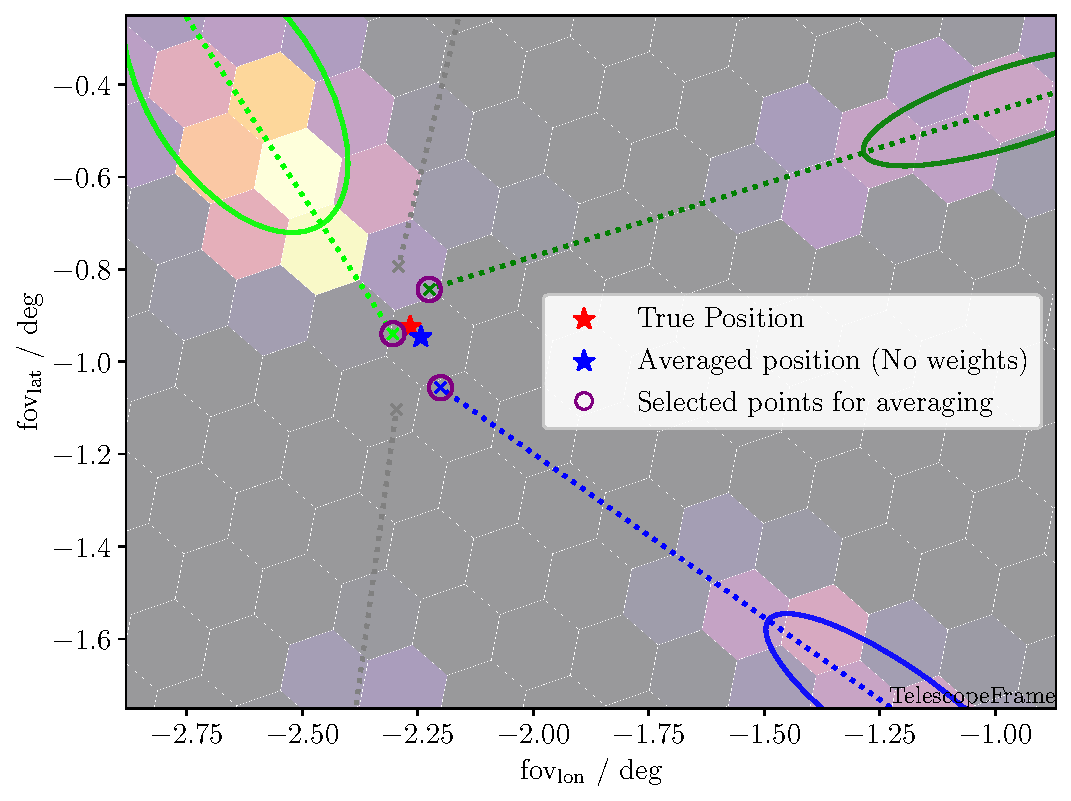
\includegraphics[width=\textwidth]{images/QualityCombiner.pdf}
      \vspace{1mm}
      {\footnotesize Illustration of the Quality-Ranked DISP combination approach.}
    \end{column}
  \end{columns}
\end{frame}

\begin{frame}{K-Means DISP Combiner}
  \begin{columns}[c, totalwidth=\textwidth]
    % Left column: explanation
    \begin{column}{0.4\textwidth}
      \begin{itemize}
        \setlength{\itemsep}{0.35cm} % increase space between items
        \item Generate \textbf{two candidates} per telescope (head and tail).  
        \item Apply \textbf{K-Means clustering} with \(N + 1\) clusters.  
        \item Incorrect points form small or isolated clusters.  
        \item Final direction = weighted average of the \textbf{largest cluster}.  
      \end{itemize}
    \end{column}

    % Right column: large image
    \begin{column}{0.59\textwidth}
      \centering
      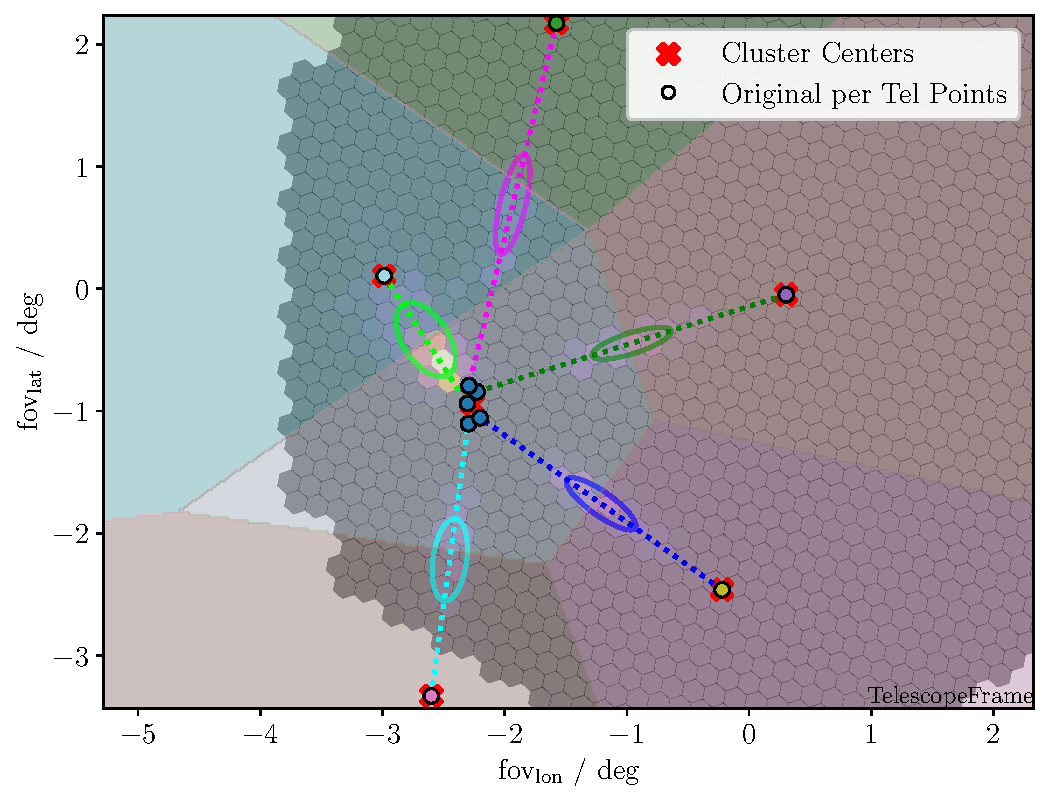
\includegraphics[width=\textwidth]{images/KMeans_fullView.pdf}
      \vspace{1mm}
      {\footnotesize Visualization of K-Means clustering on telescope predictions.}
    \end{column}
  \end{columns}
\end{frame}



\section{Results}
\begin{frame}{Results: Angular Resolution}
  \begin{columns}[c, totalwidth=\textwidth]
    % Left column: concise text
    \begin{column}{0.45\textwidth}
      \begin{itemize}
        \setlength{\itemsep}{0.5cm} % increase space between items
        \item Measure: \textbf{68\% containment radius} of angular error.  
        \item New combiners achieve up to \textbf{30\% improvement} compared to the HillasReconstructor.  
        \item Strongest gains at both \textbf{low and high energies}. 
        \item Weights for ranking and averaging as well as parameter K where optimized for the 1802884 valid events present.
      \end{itemize}
    \end{column}

    % Right column: large image
    \begin{column}{0.55\textwidth}
      \centering
      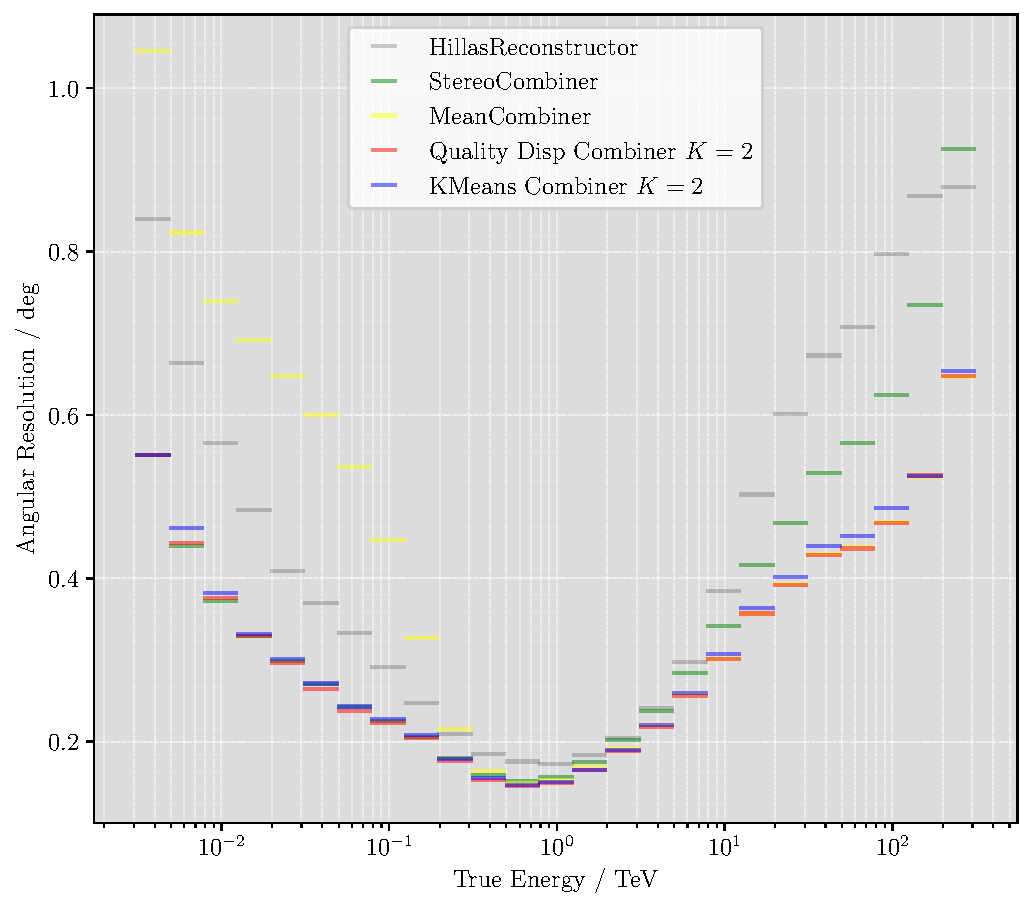
\includegraphics[width=0.9\textwidth]{images/money_plot.pdf}
      \vspace{0mm}
      {\footnotesize Comparison of angular resolution across energies.}
    \end{column}
  \end{columns}
\end{frame}


% ------------------------
\section{Outlook \& Conclusion}

\begin{frame}{Outlook}
  \begin{columns}[c, totalwidth=\textwidth]
    % ----- Left: key points -----
    \begin{column}{0.48\textwidth}
      \begin{itemize}
        \setlength{\itemsep}{0.4cm} % increase space between items
        \item Apply methods to \textbf{CTAO South} (51 telescopes).%
          \tikz[remember picture,baseline] \node (b1) {};
        \item Validate on \textbf{real observational data}.%
          \tikz[remember picture,baseline] \node (b2) {};
        \item Explore \textbf{adaptive weighting} with sign probabilities.%
          \tikz[remember picture,baseline] \node (b3) {};
        \item Add combiners into current CTA Pipe Software with \textbf{parallel} processing.
      \end{itemize}
      \vspace{2.7cm}
      {\footnotesize Images adapted from Wikipedia Observational astronomy and CTAO Website}
    \end{column}

    % ----- Right: circular PDFs -----
    \begin{column}{0.52\textwidth}
      \begin{tikzpicture}[remember picture]
        % Top circle: CTAO South config PDF
        \node (img1) at (0,0) {%
          \begin{tikzpicture}
            \clip (0,0) circle (1.8cm);
            \node at (0,0) {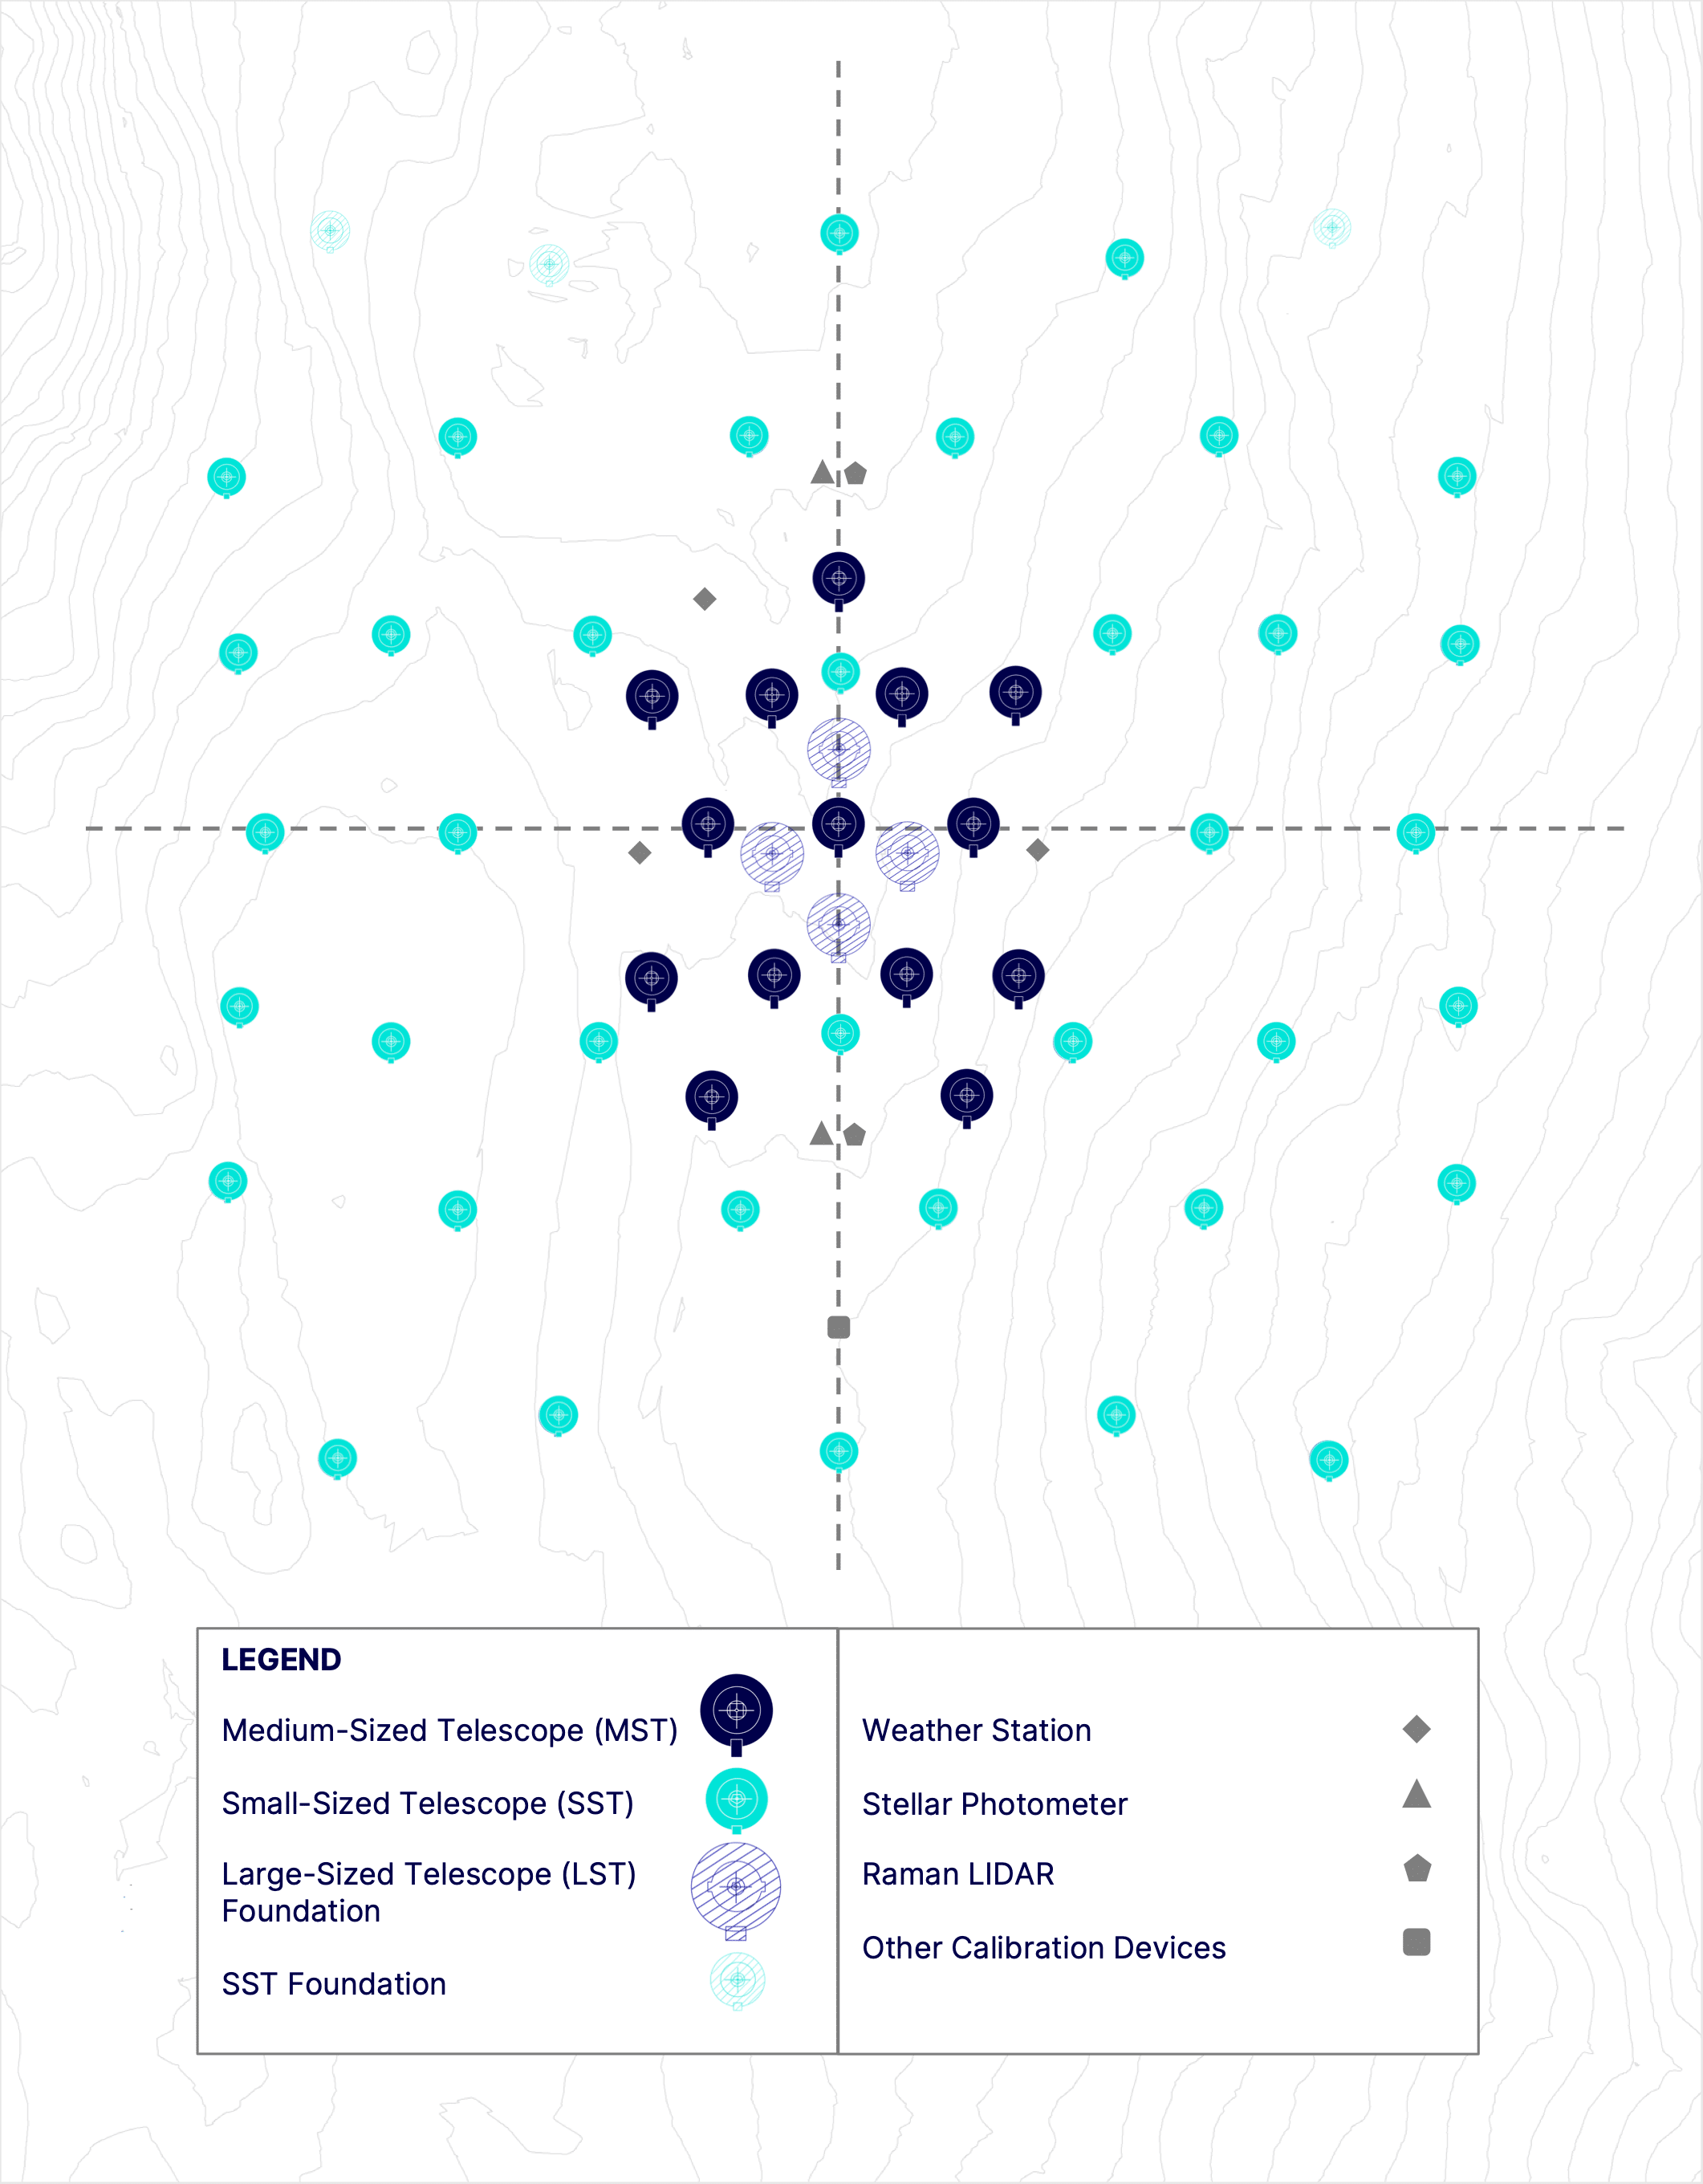
\includegraphics[page=1,width=4.0cm]{images/ctao_south.png}};
          \end{tikzpicture}
        };
        \node[below=-1cm of img1, xshift=-3.5cm] (img2) {%
          \begin{tikzpicture}
            \clip (0,0) circle (1.8cm);
            % TODO: replace placeholder with your second PDF
            \node at (0,3) {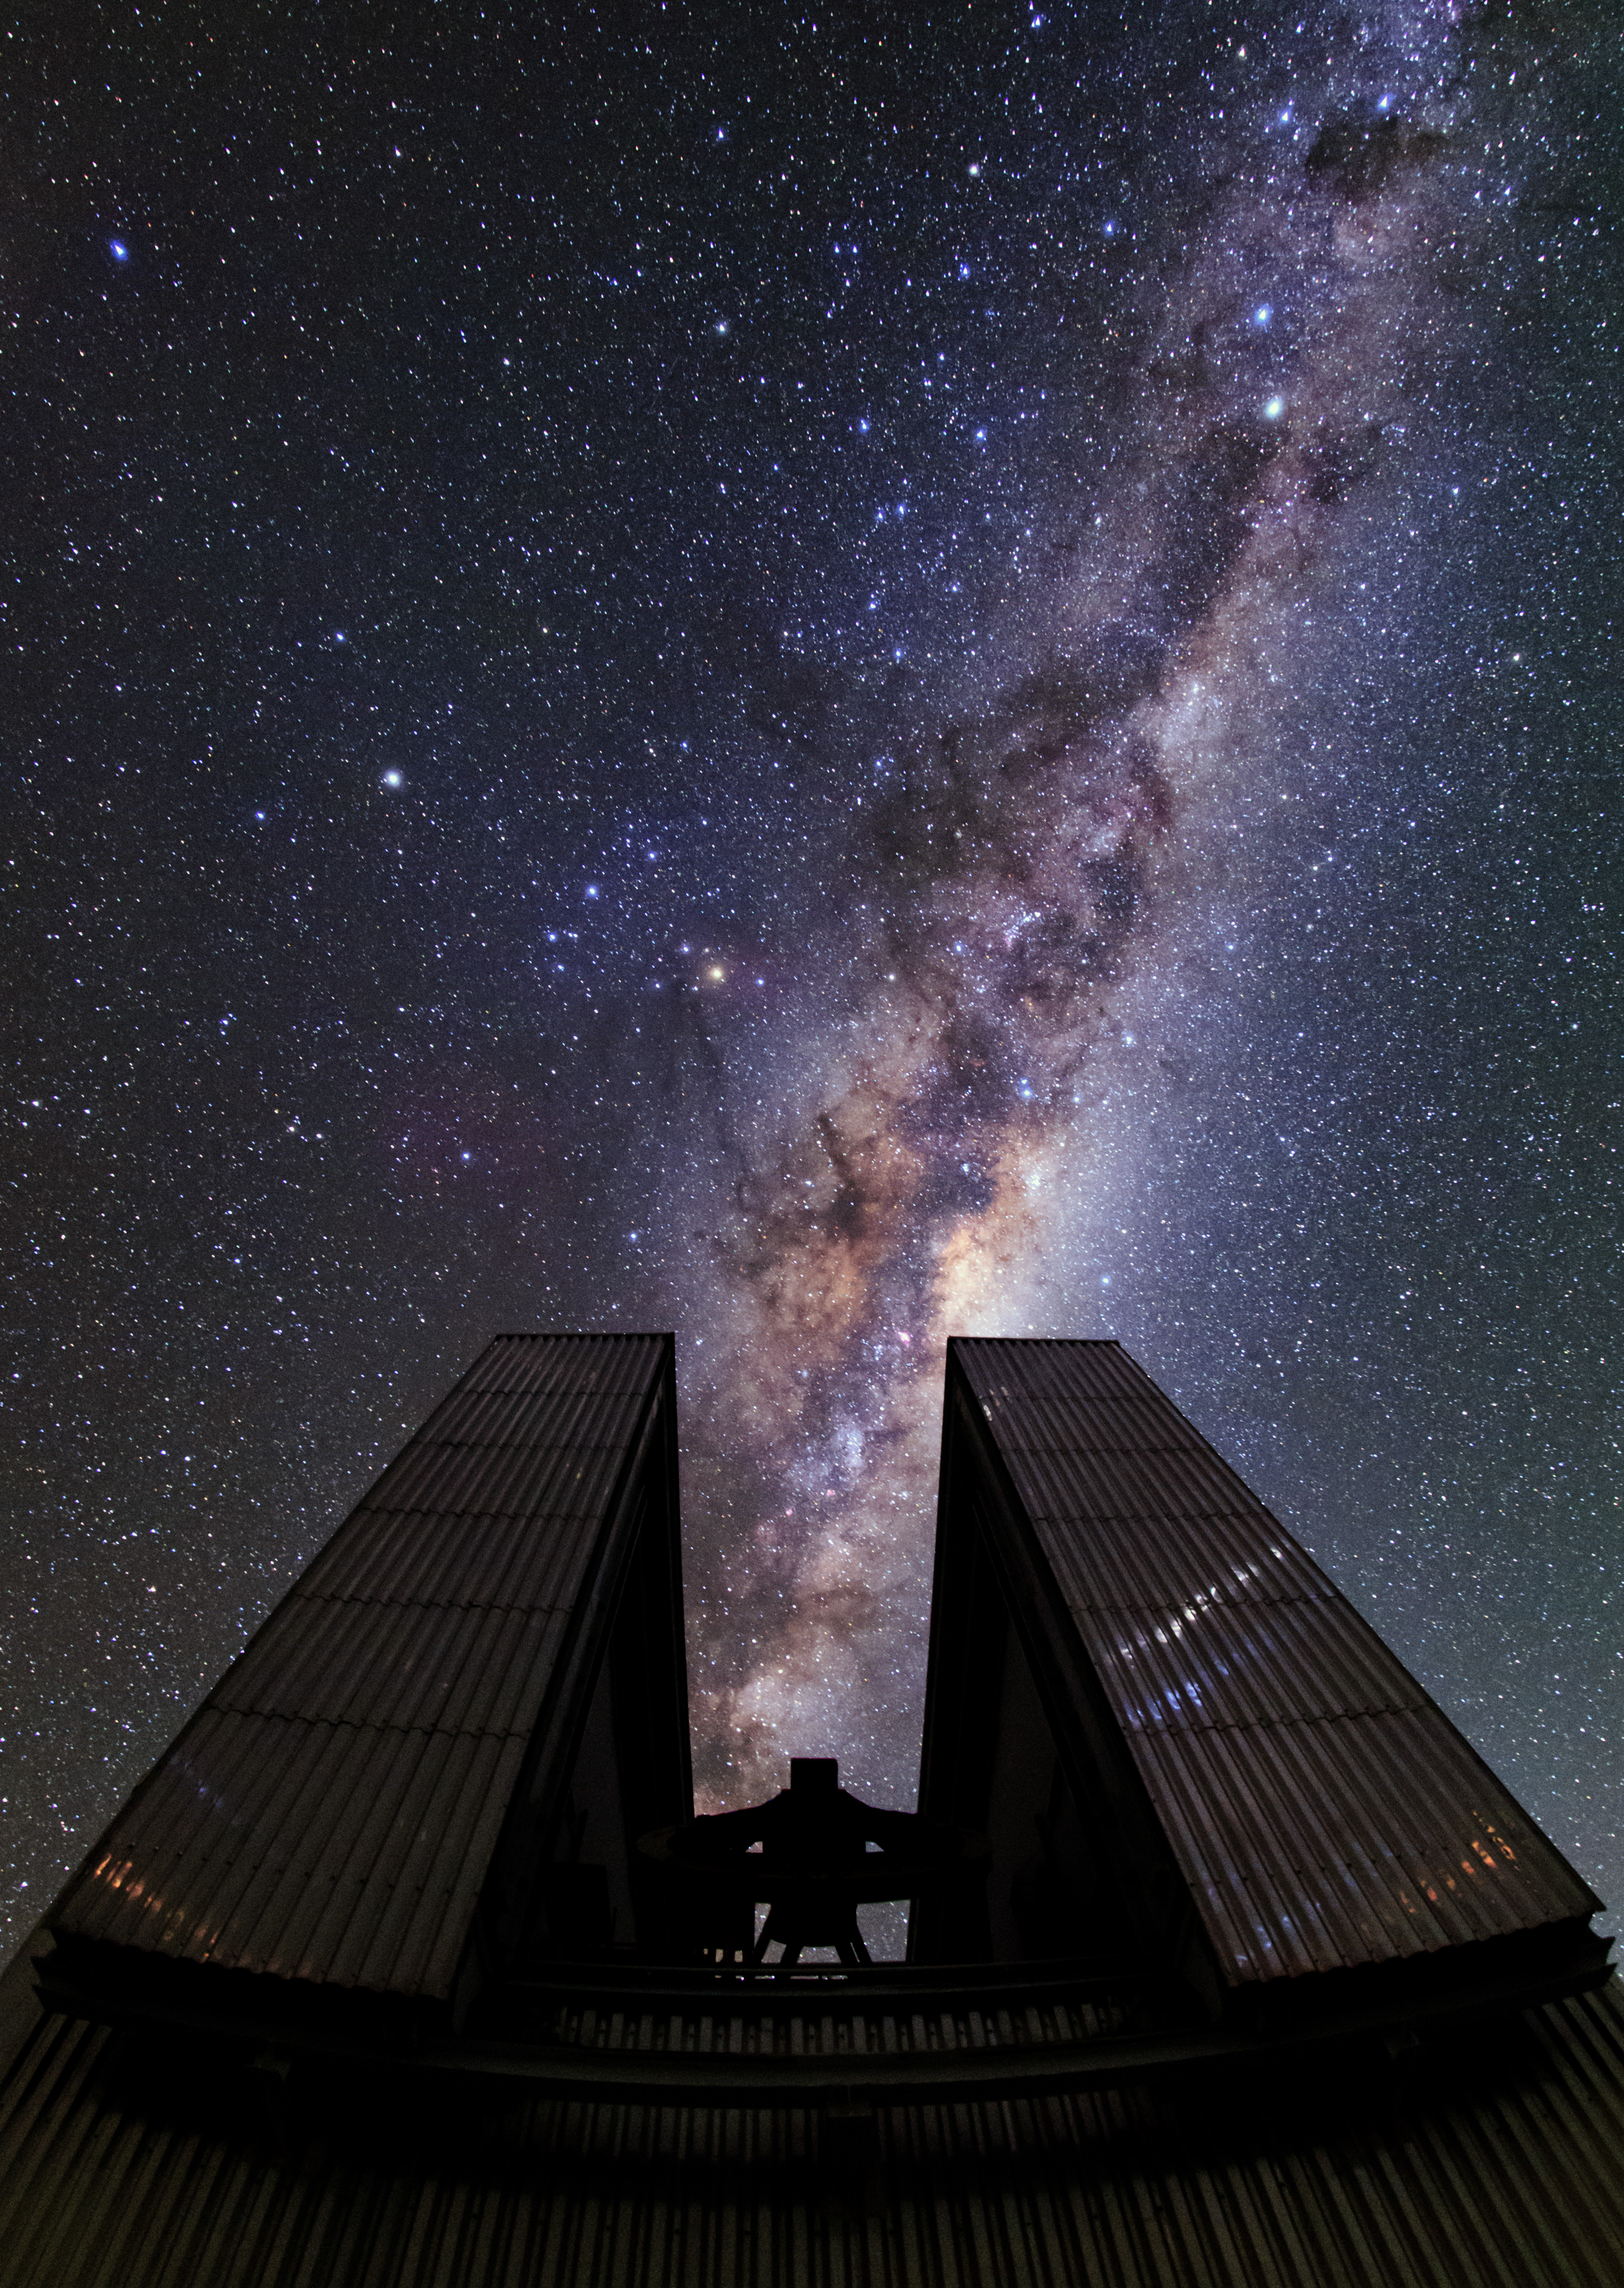
\includegraphics[page=1,width=4.0cm]{images/real_data.jpg}};
          \end{tikzpicture}
        };
      \end{tikzpicture}
    \end{column}
  \end{columns}

  % ----- Overlay arrows from bullets to circles -----
  \begin{tikzpicture}[remember picture,overlay,>=Latex]
    \draw[->,thick] (b1.east) .. controls ($(b1.east)+(1.0,0.2)$) .. ($(img1.west)+(0,0.3)$);
    \draw[->,thick] (b2.east) .. controls ($(b2.east)+(1.5,0.2)$) .. ($(img2.north)+(-0.3,0)$);
    % If you want the third bullet to point to the lower circle as well, uncomment:
    % \draw[->,thick] (b3.east) .. controls ($(b3.east)+(1.0,-0.2)$) .. ($(img2.west)+(-0.3,-0.2)$);
  \end{tikzpicture}
\end{frame}

\begin{frame}{Conclusion}
  \begin{columns}[c, totalwidth=\textwidth]
    % ----- Left: key points -----
    \begin{column}{0.48\textwidth}
      \begin{itemize}
        \setlength{\itemsep}{0.1cm} % increase space between items
        \item Gamma rays are detected through Cherenkov light with Cherenkov telescopes and need combination algorithms.%
          \tikz[remember picture,baseline] \node (b1) {};
        \item This thesis yielded improved algorithms (QualityDisp, K-Means) that improve direction reconstruction.%
          \tikz[remember picture,baseline] \node (b2) {};
        \item Better accuracy → sharper gamma-ray sky maps → deeper insights into the universe.%
          \tikz[remember picture,baseline] \node (b3) {};
      \end{itemize}

      \vspace{4mm}
      \centering
      % img3 UNDER the text (left column)
      \begin{tikzpicture}
        \node[circle, minimum size=3.6cm, inner sep=0pt,
              path picture={
                \node at (path picture bounding box.center)
                  {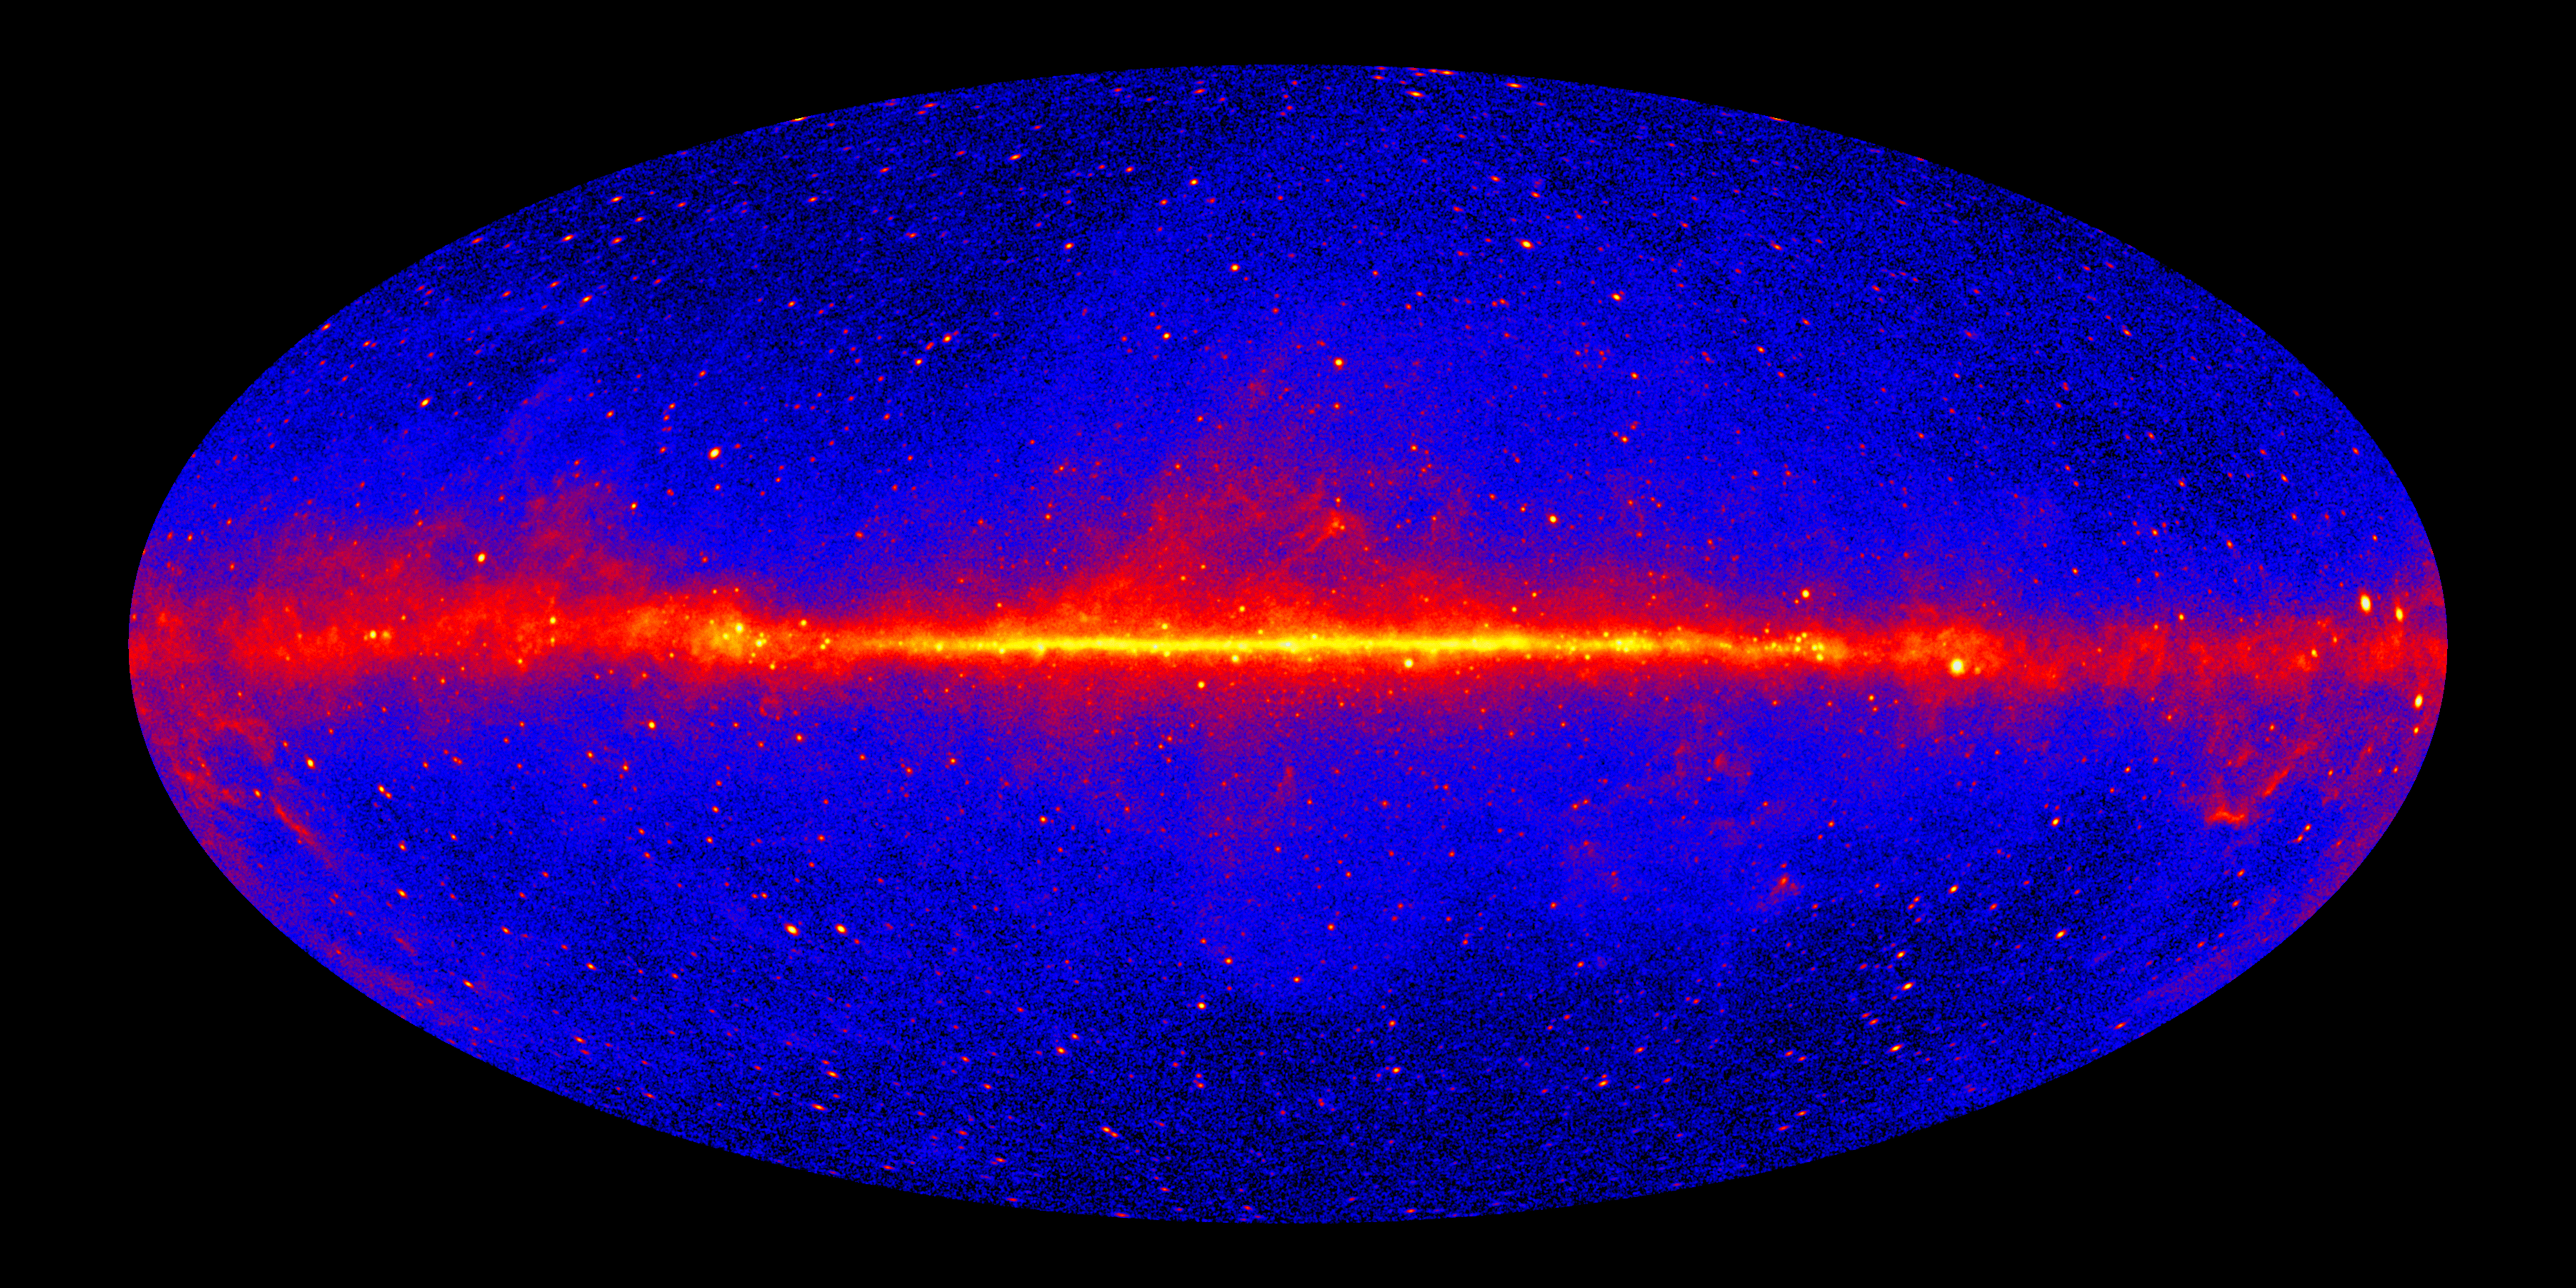
\includegraphics[page=1,width=7.2cm]{images/gamma_ray_sky.png}};
              }] (img3) {};
      \end{tikzpicture}
    \end{column}

    % ----- Right: circular PDFs -----
    \begin{column}{0.8\textwidth}
      \begin{tikzpicture}[remember picture]
        % Top circle: CTAO South config PDF
        \node (img1) at (0,0) {%
          \begin{tikzpicture}
            \clip (0,0) circle (1.8cm);
            \node at (0.5,0.5) {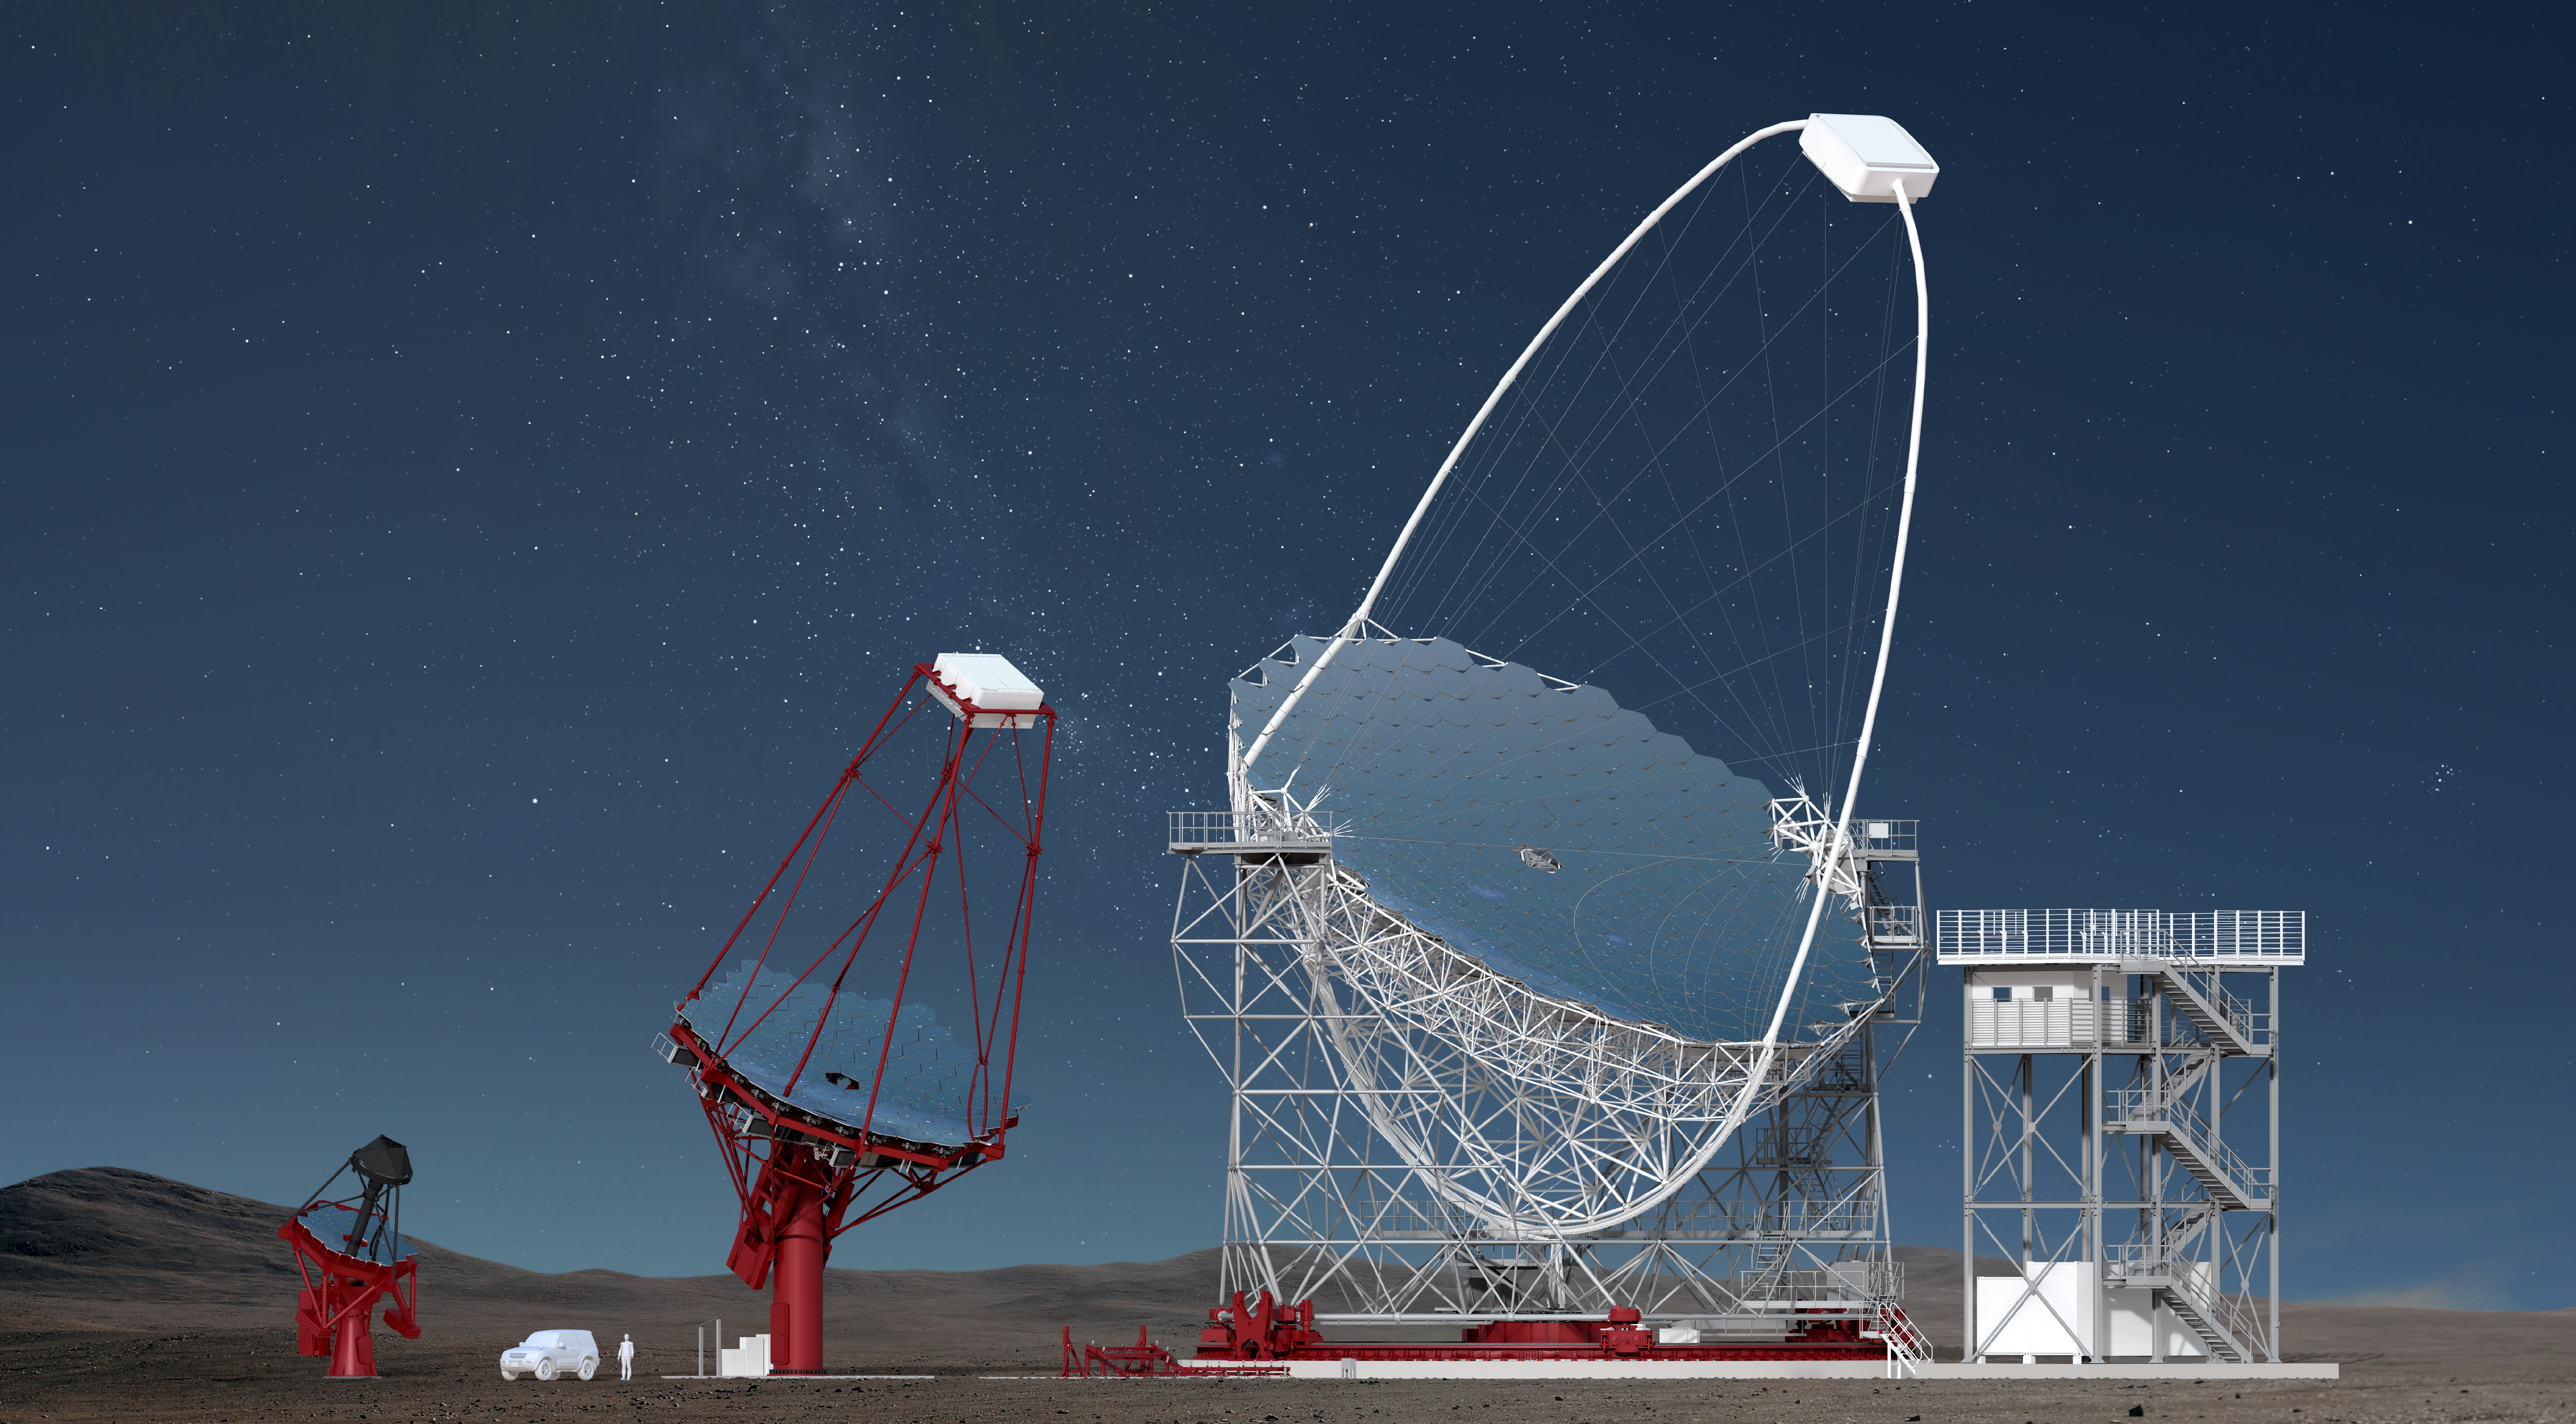
\includegraphics[clip, trim=0cm 0cm 3cm 0cm, width=5cm]{images/all_telescopes.jpg}};  
          \end{tikzpicture}
        };
        \node[below=-1cm of img1, xshift=-3.5cm] (img2) {%
          \begin{tikzpicture}
            \clip (0,0) circle (1.8cm);
            % TODO: replace placeholder with your second PDF
            \node at (0,4) {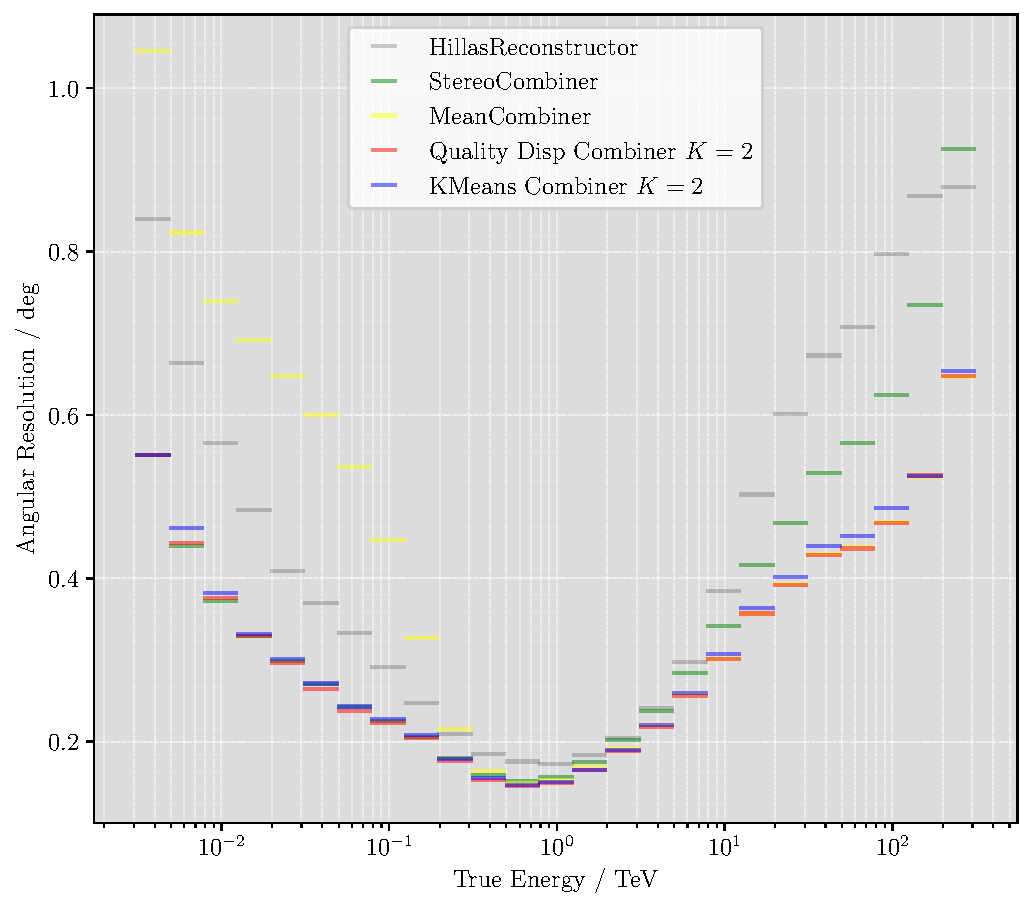
\includegraphics[page=1,width=6.0cm]{images/money_plot.pdf}};
          \end{tikzpicture}
        };
      \end{tikzpicture}
      \newline
      {\footnotesize Image sources: www.flickr.com/photos/ctao-universe and svs.gsfc.nasa.gov/14090/}
    \end{column}
  \end{columns}

  % ----- Overlay arrows from bullets to circles -----
  \begin{tikzpicture}[remember picture,overlay,>=Latex]
    \draw[->,thick] ($(b1.east)+(4.8,0.5)$) .. controls ($(b1.east)+(4.8,0.5)$) .. ($(img1.west)+(0,0.3)$);
    \draw[->,thick] ($(b2.east)+(0.5, 0.35)$) .. controls ($(b2.east)+(1.5,0.2)$) .. ($(img2.north)+(-0.3,0)$);
    \draw[->,thick] ($(b3.east)+(0.3, 0.1)$) .. controls ($(b3.south)+(1.0,-0.2)$) .. ($(img3.east)+(4,3.5)$);
  \end{tikzpicture}
\end{frame}

\section*{Backup}

\begin{frame}{Backup: Sign Regressor (LSTs Only)}
  \begin{columns}[c, totalwidth=\textwidth]
    \begin{column}{0.55\textwidth}
      \begin{itemize}
        \setlength{\itemsep}{0.6cm} % increase space between items
        \item The histogram shows the \textbf{sign prediction accuracy} per energy bin.  
        \item For higher energies, the accuracy of the sign regressor \textbf{increases steadily}.  
        \item Results shown here are for the \textbf{Large-Sized Telescopes (LSTs)}.  
        \item Medium-Sized Telescopes (MSTs) exhibit a \textbf{similar trend}.  
      \end{itemize}
    \end{column}
    \begin{column}{0.45\textwidth}
      \centering
      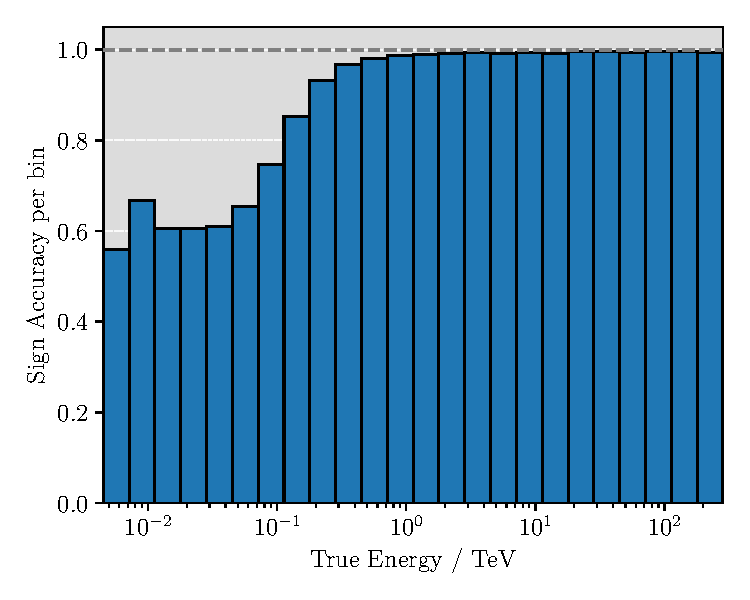
\includegraphics[width=\textwidth]{images/signregressor.pdf}
      \vspace{2mm}
      {\footnotesize Accuracy of sign regressor vs. energy (training data).}
    \end{column}
  \end{columns}
\end{frame}

\begin{frame}{Backup: Angular Resolution Comparison}
  \begin{columns}[c, totalwidth=\textwidth]
    \begin{column}{0.5\textwidth}
      \centering
      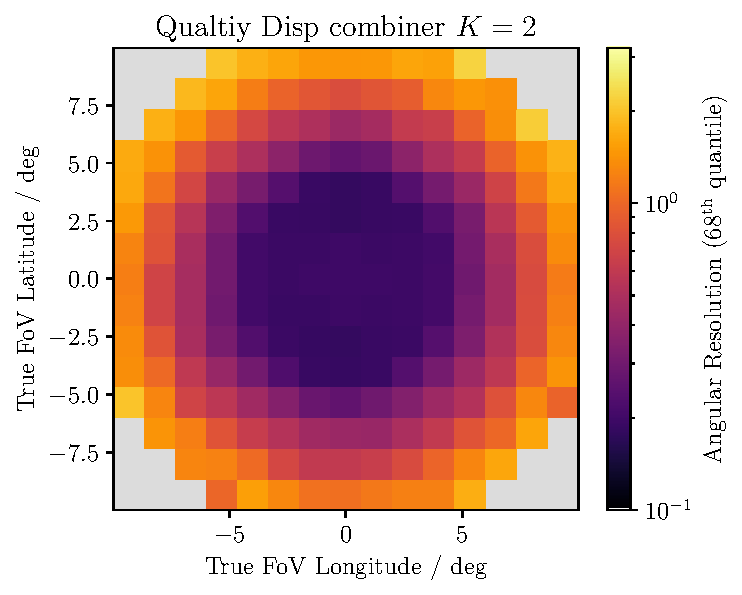
\includegraphics[width=\textwidth]{images/AngularPlot_2QualtiyDisp.pdf}
      \vspace{2mm}
      {\footnotesize QualityDisp combiner: improved angular resolution across energies.}
    \end{column}
    \begin{column}{0.5\textwidth}
      \centering
      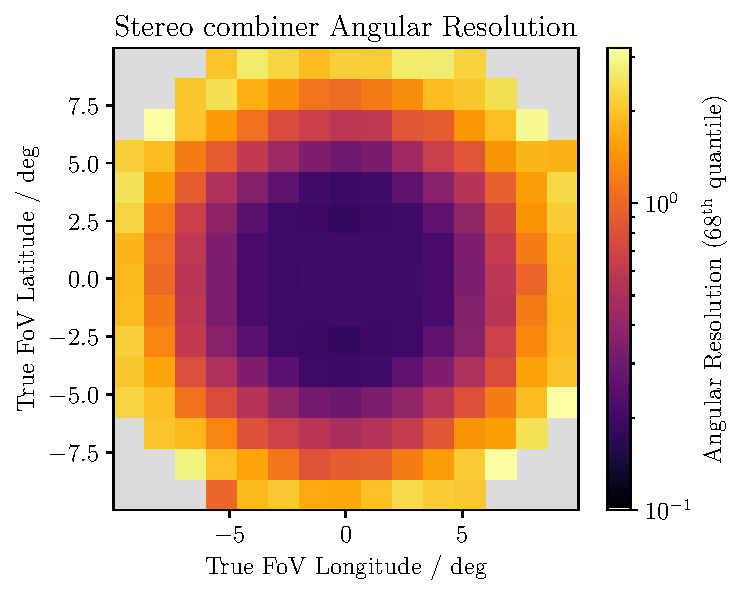
\includegraphics[width=\textwidth]{images/AngularPlot_Stereo.pdf}
      \vspace{2mm}
      {\footnotesize Stereo combiner: shows degradation toward outer image regions.}
    \end{column}
  \end{columns}
  \vspace{4mm}
  \small
  The \textbf{stereo combiner} degrades more strongly at the image edges  
  as the \textbf{QualityDisp combiner} due to higher energies.
\end{frame}

\begin{frame}{Backup: QualityDisp Variants}
  \centering
  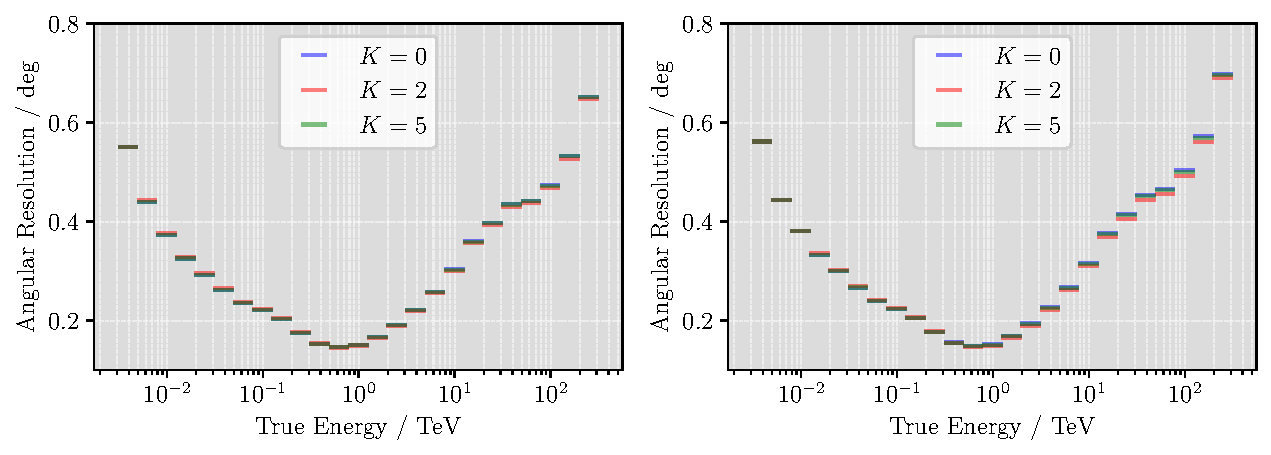
\includegraphics[width=0.8\textwidth]{images/quality_disp_left_konrad_right_intensity.pdf}
  \vspace{3mm}

  \begin{itemize}
    \item \textbf{Left plot:} uses the \textbf{Conrad parameter} for averaging.  
    \item \textbf{Right plot:} uses the \textbf{intensity} as the averaging weight.  
    \item Both approaches apply \textbf{Conrad weights} for telescope ranking.  
  \end{itemize}

  \vspace{3mm}
  {\footnotesize Further parameter optimization may yield improved performance,  
  especially for the \textbf{CTAO South site} with its higher number of telescopes.}
\end{frame}

\end{document}

%https://www.flickr.com/photos/ctao-universe/albums/72157672713462861/with/50248188932 Hier gibt es ein paar Bilder

